%%===================================
\documentclass[12pt]{article}
\usepackage{ramsstyle}
\renewcommand\contentsname{Innhold}
\renewcommand\refname{Referanser}
\renewcommand\bibname{Bibliografi}
\renewcommand\figurename{Figur}
\renewcommand\listfigurename{Figurliste}
%%===================================
\begin{document}
%This is the Titlepage
%%=========================================
\thispagestyle{empty}
%
\includegraphics[scale=1.1]{fig/rams}
\mbox{}\\[6pc]
\begin{center}
\Huge{Intelligente Brukergrensesnitt i Smarte Hjem}\\[1pc]

\Large{- Hvordan tilby naturlig og effektiv interaksjon?}
\\[2pc]

\Large{Andreas Arning Flakstad}\\[1pc]
\large{Vår 2015}\\[2pc]

TDT4501 - Masteroppgave\\
Institutt for datateknikk og informasjonsvitenskap\\
Norges teknisk-naturvitenskaplige universitet
\end{center}
\vfill

\noindent Veileder: Ass. Prof. Asbjørn Thomassen



\setcounter{page}{0}
\pagenumbering{roman}
%This is the Preface
%%=========================================
\addcontentsline{toc}{section}{Forord}
\section*{Forord}
Hva er masteroppgave..\\[2cm]

%This is the Acknowledgment
%%=========================================
\addcontentsline{toc}{section}{Anerkjennelse}
\section*{Anerkjennelse}
Maya, Asbjørn, ..

%%=========================================
\addcontentsline{toc}{section}{Sammendrag og konklusjoner}
\section*{Sammendrag og konklusjoner}
asd

\listoffigures
\newpage
\tableofcontents
\newpage
\setcounter{page}{0}
\pagenumbering{arabic}
%%=====================================
%%=========================================
\section[Introduksjon]{Introduksjon}
%%=========================================
\subsection{Bakgrunn}

\subsubsection{Smarte hjem}
Definisjon. Behovet for smarte hjem: informasjon, læring, kommunikasjon, energieffektivitet, støtte av eldre.

Ideén om et smart hjem refererer i følge \citet{peine08} til å bruke informasjons- og kommunikasjonsteknologi (IKT) i hjemmet for å forenkle interoperabilitet av husholdningsprodukter og tjenester. Peine skriver at ideén har vært beskrevet siden 80-tallet og har i de senere år fått en ny interesse i industrien. Faktisk har kontroll av funksjonaliteten i en kontorbygning eksistert siden 70-tallet, med muligheter for å kontrollere lys, varme, elektristet og adgangskontroll fra et sentralt sted. Det tok noen år før man innså at de samme egenskapene kunne være ønskelige å implementere for å automatisere hus. Den sentrale forskjellen mellom et vanlig hus og smart hus er denne muligheten for å styre flere aspekter ved huset gjennom en sentral enhet.

På markedet finnes det nå flere løsninger for å automatisere deler av hjemmet eller tilby gode brukergrensesnitt for å styre funksjonalitet som lys og varme. Disse løsningene bidrar med å ivareta sikkerhet og hjelper til å begrense energiforbruket. De tilbyr gjerne informasjon om hjemmet via en mobilapplikasjon så man kan ha oversikten selv når man er bortreist. Ved å benytte enheter som er tilknyttet internettet, som termostater, lys, låser, sikkerhetssystemer og garasjeporter, kan man styre dem gjennom mobilapplikasjonen\footnote{Et søk i Google på "smarthome" og norske resultater gir for eksempel denne hjemmesiden der en privatperson har tatt i bruk og satt sammen komponenter fra markedet for å skape en helhetlig og gjennomført løsning: http://www.samdal.com/SmartHome.htm}. Disse løsningene er svært praktiske og gir god verdi, men er økt tilgang til informasjon og muligheten til å fjernstyre noen deler av hjemmet det beste vi kan få til i dag?

I en artikkel for Scientific American i 1991 skrev Mark Weiser at de mest dyptgripende teknologiene er de som forsvinner inn i hverdagslivet inntil det er umulig å skille dem ut igjen. Han så for seg at omgivelsene var gjennomtrengt med teknologi for databehandlig og kommunikasjon, og som kunne støtte opp under menneskers liv gjennom såkalt \emph{calm computing} \citet{weiser91}. Dette framtidssynet har styrt utviklingen for forskningsområdene \emph{pervasive/ubiquitous computing} og det peker mot de egenskapene og mulighetene et smart hjem bør tilby. Men hvorfor er ikke smarte hjem smarte nok til å tilby dette framtidssynet ennå? Det har godt mange år og det har blitt gjort mye arbeid siden 1991. Trolig har vi all del-funksjonaliteten som trengs for å implementere dette framtidssynet. Vi har kraftige innebygde enheter, sensorer på størrelse med frimerker, trådløs kommunikasjon, internettet og muligheten til å programmatisk kontrollere elektriske apparater, varme og lys. Vi kan analysere bilder og lydsignaler, gjenkjenne fjes og tale, overvåke og følge brukerenes bevegelser, samt koble oss opp mot eksterne datakilder som værmeldinger og brukerenes kalendere. Grunnen til at vi ikke har disse systemene ennå må være at det er vanskelig å sette det hele sammen og å gjøre god bruk av alle dataene som samles inn. Kunstig intelligens kan være nøkkelen for å gjøre teknologiene vi har om til nyttige tjenester.

For å forstå omgivelsenens tilstand vil det være nødvendig å analysere sensorinformasjon. To lovende input-kanaler er lyd og bilde. Ettersom vi mennesker kommuniserer med tale er det naturlig at et AmI-system skal kunne håndtere dette. Talegjenkjenning er et vanskelig problem, men det er et område det er jobbet mye med opp gjennom årene. Ved bruk av teknikker fra signalprosessering og mønstergjenkjenning kan man identifisere \emph{fonemer} i signalet og deretter ord. Tilsvarende kan man få en datamaskin til å utnytte seg av syn ved å få tak i input som bilder. Disse må også prosesseres og mennesker må gjenkjennes. I følge \citet{augustonugent06} kan datasyn kan være nyttig for å gjenkjenne mønstre i menneskers oppførsel eller oppdage når noe galt har skjedd, som at en eldre beboer har falt. Det kan også brukes til å gjenkjenne gesturer eller å gjenkjenne fjesuttrykk i et forsøk på å forstå brukerenes følelser. Dersom datasyn skal brukes vil det være viktig å skille beboeren fra besøkende, dyr eller andre bevegelige objekter. Å holde en historie over beboerens siste bevegelser kan hjelpe til med å forstå og avgjøre tilstander.

Et virkelig smart hjem kan lære av å observere brukere. Teknikker fra maskinlæring, som nevrale nettverk, case-based resonnering og beslutningstrær og støttevektormaskiner er godt utviklet og kan benyttes til dette. Å lære brukernes oppførsel vil være essensielt for at system skal forbedre seg selv over tid, og for å tilby en individuelt tilpasset opplevelse. Forskjellige brukere vil ha forskjellige tilstander, preferanser og vaner, og disse bør tas med i beregningen for at systemet skal være verdifullt.

Data som hentes fra hjemmet kan være interessant for forskjellige brukere, men hvilken informasjon skal hver person motta? Her kommer privathet og sikkerhet inn i bildet. Hvordan og til hvilket tidspunkt tar vi kontakt med brukeren? Uønsket eller unødvendig hjelp er sannsynligvis verre enn ingen hjelp. Påminnelser om oppgaver med lav prioritet kan være frustrerende. Vi ønsker kanskje heller ikke at brukere blir overavhengige av systemet, selv hvis det fungerer godt. For mange brukere kan dette peke mot at vi ønsker et minimalt nivå av hjelp. Dette vil la beboern ta i bruk sin egen kognitive kapasitet og vedlikeholde et høyt nivå av uavhengighet. 


\subsubsection*{Hva ønsker brukerne}
Ettersom vi snakker om hvorfor og hvordan man vil utvikle løsninger for å skape smarte hjem kan det være en god idé å ha kontakt med brukermassen. Smarte hjem er et relativt nytt produkt for det store markedet, så det er ikke sikkert at brukerene vet hva de vil ha fra et smart hjem, eller om de vil ha et smart hjem i det hele tatt. Men ettersom dette kan sees på som utviklingen av et nytt produkt vil det allikevel være klokt å ta pulsen på framtidige kunder. I stedet for å dytte behov på brukeren kan det være bedre å støtte opp under brukerens faktiske behov. Dette kan hjelpe oss å bygge produkter som blir godt motatt og dermed kan vi framskynde innføringen av smarte og automatiserte hjem.

\citet{bonino11} ledet en interessant italiensk studie som spurte en gruppe hva de ville spurt hjemmet sitt dersom det var intelligent. Studien viser at folk flest har sterke følelser knyttet til hjemmet. Det er et trygt og koselig sted. Det er et sted til å stole på og følelsen av å returnere dit er god. Generelt er å føle seg bra en del av hjemopplevelsen. Atmosfæren er behagelig og tilpasset brukerens preferanser og folk liker at de kan gjøre hva de selv vil. Brukere har følelsen av å være i kontroll.

Artikkelen presenterer hva gruppen mener er de viktigste områdene for det smarte hjemmet:
\begin{itemize}
  \item Intelligente brukergrensesnitt på hvitevarer, for eksempel stemmekontrollerte oppvaskmaskiner.
  \item En tilgjengelig klokke, for planlegging av aktiviteter.
  \item Tilgang til værinformasjon, da ønskede fritidsaktiviteter ofte avhenger av været utendørs.
  \item Ivaretagelse av egen sikkerhet og husets sikkerhet. Innbruddsbeskyttelse og automatisk oppdagelse av farer, som røyk-, varme- eller gassutvikling.
  \item Informasjon om energiforbruk og forslag til hvordan energiforbruket kan reduseres.
  \item Kontroll av husets underholdningssenter.
  \item Tilgjengelig kommunikasjonsbehov som å lese epost og bruke telefon.
  \item Automatisk oppdagelse og eventuell reparasjon av problemer.
  \item Husholdningsoppgaver som hjelp med oppgaver til å holde huset rent og komfortabelt, håndtering av mat og hjelp med planlegging av innkjøp.
  \item Komfortrelaterte problemer som lysregulering, temperaturregulering og operering av vinduer og persienner.
  \item Personlig assistanse, som å be huset om hjelp til å huske ting, søke opp informasjon og håndtere andre dagligdagse oppgaver.
\end{itemize}

En annen studie av brukerbehovene for smarte hjem presenteres av \citet{userreq}. Her omtales en empirisk studie utført på seks forskjellige steder i fem europeiske nasjoner. Studien bruker en scenario-drevet tilnærming og brukte kvantitative og kvalitative metoder for å få tilbakemelding fra brukermassen om konsepter innen smarte hjem. Deltakerene kom opp med en rekke forslag og ideer til hva et smart hjem bør tilby og prioriteringsrekkefølgen for disse funksjonalitetene. Generelt ble det funnet godt med beviser på hva brukere er interessert i: Systemet skal være lett å bruke og å konfigurere. Det skal ikke kreves programmering eller vedlikehold av noe slag. Systemet skal være modulært og tilby å justere for individuelle preferanser. Alle deltakerene var enig om at personvernet ikke måtte brytes gjennom overvåking. Den følgende listen er sortert med høyeste prioritet først.
\begin{enumerate}
  \item Brukeren må alltid være i kontroll av systemet.
  \item Systemet må ivareta sikkerhet, og beskytte personvernet.
  \item Et nytt system må gi ny verdi over eksisterende systemer.
  \item Systemet må ikke unødvendig overta rollen til direkte kommunikasjon mellom mennesker.
  \item Hjemmekomforten skal alltid ivaretas.
  \item Systemet skal tilby passende informasjon til passende brukere på forskjellige lokasjoner basert på brukerpreferanser.
  \item System skal redusere tiden som trengs for å utføre husholdningsoppgaver som vasking.
  \item Systemet skal integrere og kombinere funksjonaliteten til hvitevarer.
  \item Systemet skal være energibesparende.
  \item Systemet skal være kostnadsbesparende.
  \item Systemet skal støtte organiseringsaktiviteter og planlegging for flere personer i hjemmet, mellom forskjellige hjem og mellom hjemmet og jobb.
  \item Systemet skal beskytte mot datatyveri og annen manipulering (se punkt 2).
  \item Systemet skal tilby adgangskontroll og respektere individuelle preferanser og autoriteter.
  \item Systemet skal holde informasjon om kontekst og omgivelsene.
  \item Systemet skal forholde seg til implisitte sosiale normer.
  \item Systemet skal beskytte personvernet til enhver tid (se punkt 2).
\end{enumerate}

\subsubsection*{Støtte av eldre og funksjonshemmede}
Smarte hjem ønsker å tilby funksjonalitet relatert til gevinst innen økonomi og komfort, som at lys og varme skrues av og på automatisk avhengig av beboernes tilstedeværelse. Men det kan argumenteres for at den viktigste funksjonaliteten er for å forbedre en uavhengig livsstil for eldre og funksjonshemmede. Basert på antallet artikler om teamet må å opprette støtte for at eldre og funksjonshemmede skal få leve uavhengig i lengre tid være en av de mest studerte tilnærmingene til smarte hjem. En god grunn er at dette er den gruppen mennesker som vil ha størst nytte av et smart hjem. Muligheten til å fortsette å leve uavhengig og selvstendig i sitt eget hjem, framfor å bli innlagt på en institusjon, er virkelig verdifull. Et smart hjem kan hjelpe til med funksjonalitet som å gi påminnelser om at medisin må tas og å oppdage dersom noe har gått galt og automatisk ta kontakt med hjelpetjenester eller familie.

Den andre gode grunnen til at denne tilnærmingen studeres mye er på grunn restriksjonene denne beboergruppen har i sitt levesett. Når de forskjellige aktivitetene beboerne utfører kan telles på noen få hender blir det store problemet om å få et datasystem til å forstå menneskelige aktiviteter mye enklere. Det blir satt restriksjoner på problemet som gjør at det faktisk kan løses. Å løse problemet uten restriksjoner kan vise seg å være en svært vanskelig og kanskje umulig oppgave. Vi mennesker gjør ofte flere aktiviteter på en gang, samarbeider med andre mennesker og vi kan avslutte aktiviteter midtveis.


\citet{desilva12} påpeker at for systemene som fokuserer på støtte av eldre og funksjonshemmede er det ekstra viktig å detektere mennesker, ettersom en av hovedfunksjonalitetene til et slikt system er å gjenkjenne hvilken tilstand beboeren er i. Dersom beboeren for eksempel har falt er det viktig å gjenkjenne objektet på bakken som et menneske og ikke som en livløs gjenstand. Ettersom å gjenkjenne mennesker er av høyeste prioritet benytter mange av prosjektene i denne kategorien videoovervåkning. Når det gjelder deteksjon av fall skriver \citet{elliot09} om bruken av en pendel, refleksjons-sensorer og et nevralt nettverk for å følge pendelens posisjon i reell-tid. Resultatene indikerte at teknikken er tilstrekkelig sensitiv og kan brukes til å gjenkjenne forskjellene mellom en person som finner balansen og en som er i ferd med å falle. På denne måten kan hjemmet gjenkjenne og potensielt forhindre et fall før det skjer.

Casattenta-prosjektet gjør bruk av utplasserte sensorer, \emph{monitoring nodes}, fordelt i hjemomgivelsene, samt bærbare enheter, \emph{active keys}, for å overvåke beboernes helse og aktivitet (se figur \ref{casattenta}). \citet{casattenta} skriver at målet er å tilby tilstrekkelig, men ikke-påtrengende, overvåkning for å forbedre sikkerheten og livskvaliteten til eldre mennesker som bor alene. Omgivelsessensorene tillater overvåking av de typiske funksjonene i et avansert hjem: tilgangskontroll, gasslekkasjer, lys, lyd, åpne vinduer, fuktighet og temperatur. Interaksjonen mellom de utplasserte sensorene og de bærbare enhetene tillater innendørs sporing av menneskene og muligheten til å oppdage farlige hendelser. Sporingen realiseres ved å benytte signalstyrken mellom den bærbare enheten og sensorene i omgivelsene. Prosjektet gjorde bruk av den strømgjerrige ZigBee-protokollen for kommunikasjon mellom enhetene. Systemet kan også oppdage om uautoriserte personer befinner seg i hjemmet. Dersom en person oppdages ved en infrarød sensor og systemet ikke registrerer en bærbar enhet i det samme området kan en alarm aktiveres. Alarmen kan få brukerens bærbare enhet til å vibrere eller aktivere et web-kamera i nærheten for å tilby informasjon til slektninger eller andre. Systemet kan også detektere fall ved kombinasjonen av et akselerometer i den bærbare sensoren som kan si om personen ligger, og sporingen som kan si om personen befinner seg på soverommet eller ikke. Dersom et fall registreres kan systemet vibrere den bærbare enheten. Dersom brukeren ikke stopper alarmen går den videre og systemet tar kontakt med utenforstående og skrur på web-kamera for å tilby innsyn til hjemmet.

\subsubsection*{Energieffektivitet}
I disse dager dukker energibesparing stadig opp i den offentlige debatten. Å kutte energiforbruket er et samlet mål for mange i vår del av verden. Dette strekker seg også til hjemmet og kan blant annet oppnås ved å skru av lys og varme når det ikke trengs. Et smart hjem kan enten aktivt gå inn og skru ned eller av lys, varme og apparater når de ikke er i bruk, eller det kan overvåke energibruken og periodisk komme med forslag til forandring i brukerens holdning til bruk av elektrisitet. Et alternativ for å oppnå bedret energieffektivitet er å anvende multiagent-paradigmet og gi agentene et mål om å være energieffektive.

I kapittel to så vi på kunstig intelligens' definisjon av agenter og hvordan denne tilnærmingen kan hjelpe oss å løse problemer. Noen problemer er svært vanskelige eller umulige for en enkelt agent å løse. Her kan et multiagent-system komme inn i bildet. Dersom hjemmet er kontrollert av en gruppe agenter med forskjellige egenskaper og ansvarsområder kan de sammen potensielt løse kompliserte problemer. Nye problemer innen kommunikasjon, prioriteringer og utførelse dukker opp, men dersom disse totalt sett er enklere å løse er tilnærmingen alt i alt god. Agentene i et multiagent-system er som regel uavhengige og fokuserer på seg selv og sin oppgave. Systemet som en helhet er desentralisert og hver agent kjenner ikke til hele problemområdet. Det er derfor viktig at kommunikasjonen er god for å effektivt kunne løse problemer. En stor fordel med et slikt system er fleksibiliteten. Ettersom det er desentralisert kan nye agenter legges til og systemet som en helhet kan modifiseres uten større problemer. Dette gjør også at systemet er enklere å vedlikeholde og at det selv kan håndtere eventuelle problemer. Flere agenter som kan håndtere de samme oppgavene kan leve i systemet slik at dersom en av dem feiler håndterer den andre fremdeles oppgaven. Flere prosjekter i litteraturen har angrepet smarte hjem-problemet med multiagent-paradigmet. Jeg har lyst til å nevne to prosjekter i noe detalj.

MavHome-prosjektet (Managing An Intelligent Versatile Home) har hatt som mål å skape et hjem som oppfører seg som en rasjonell agent. \citet{mavhome} skriver at agenten forsøker å oppnå to mål samtidig: å maksimere beboernes komfort og å minimere kostandene for å operere hjemmet. For å nå disse målene må agenten ha evnen til å forutse bevegelsesmønstrene og bruken av elektriske enheter blant brukerene. Individuelle agenter kan ta seg av en del av problemet, men må koordinere deres handlinger for å oppnå det overordnede målet.

Med \emph{Thinkhome}-prosjektet påpeker \citet{thinkhome} at tidligere løsninger på smarte hjem ikke har klart å holde energinivået lavt og samtidig tilbudt god komfort for beboerne. Thinkhome benytter en stor kunnskapsbase for å ta vare på den nødvendige informasjonen for energieffektivitet og brukerkomfort, og anvender multiagent-paradigmet for å bygge et intelligent system. På samme måte som MavHome fokuserer Thinkhome på energibruk på grunnlag av økonomiske og bærekraftige mål. Samtidig prioriteres komfort ettersom nettopp dette er høyt rangert blant brukerbehovene i et automatisert hjem. Målet for prosjektet er danne en arkitektur som kan brukes i neste generasjons bygninger.

\subsubsection{Brukergrensesnitt}
Definisjon. Definisjon Intelligente Brukergrensesnitt. Definisjon naturlig og effektiv interaksjon. Design av brukergrensesnitt. Alternative interaksjonsformer. Problemer med beskyttelse av personvern.

\subsubsection*{De tre typene informasjonssystemer}
Informasjon, manipulasjon, kommunikasjon: har forskjellige krav til design.

\subsubsection*{Er brukergrensesnitt viktigere enn proaktivitet?}
I det forrige kapittelet så vi på hva brukerene ønsker seg. Noen av deres ønsker kan være vanskelig å implementere uten å bryte andre ønsker, som at systemet skal forstå konteksten i omgivelsene uten å være overvåkende. Uansett, det viktigste for de spurte gruppene var å selv være i kontroll av et systemet som var enkelt å bruke og som ga muligheter til å styre diverse deler av huset, inkludert elektriske apparater, hvitevarer, hjemmeunderholdning, lys og varme. Alt i alt er det kanskje viktigere for vanlige brukere at det tilbys gode styringsmuligheter, enn at systemet er proaktivt?

I en kontroversiell artikkel fra 2006 påpeker \citet{rogers06} at vi ennå ikke gjør "smart" på en god måte, nettopp fordi det involverer å løse svært vanskelige problemer innen kunstig intelligens . Tre områder har vært fokuset for \emph{pervasive/ubiquitous computing}: kontekstbevissthet, omgivelser som responderer til menneskelig tilstedeværelse og overvåking. Disse problemene kan på flere måter sees på som vanskeligere å løse enn det å skape et kunstig menneske. Forskningsmiljøet har møtt spesielt store problemer med den store variasjon i hva folk gjør, hvilke motiver de har, når de gjør det og hvordan de gjør det. Konteksten rundt folks dagligdagse liv er svært subtil og det i en mye større grad enn kontekstteorier har fått oss til å tro. Dette gjør det vanskelig, om ikke umulig, å implementere kontekst slik at det kan dras nyttige spådommer om hva mennesker føler, hva de ønsker eller hva de trenger i et gitt øyeblikk. Det finnes også etiske og sosiale bekymringer. I kapittel en nevnte vi Mark Weiser's drøm om \emph{calm computing}, der omgivelsene er gjennomtrengt med teknologi som støtter opp våre liv og gjør dem så komfortable som mulig. La oss si at Weisers drøm blir en virkelighet. Er dette en tilværelse vi ønsker å leve i? Bør de menneskelige kognitive prosessene druknes med en assistert levetilværelse?

Rogers foreslår en alternativ agenda. Hun argumenterer for et skifte fra proaktiv databehandling to proaktiv mennesker. Allestedsnærværende teknologier bør designes slik at brukere kan interagere med dem mer aktivt. I stedet for \emph{calm living} bør vi ønske \emph{engaged living}. Mennesker, i stedet for maskiner, bør ta initiativet til å være konstruktive, kreative og engasjere i interaksjoner. I stedet for å pakke omgivelsene med all slags forsvinnende teknologi, bør vi tenke på teknologien som et sett med verktøy og overflater som er mobile og tilrettelegger for samarbeid. Informasjonskilder, andre mennesker og omgivelsene kan sees og interageres med når det er behov for det. Videre forskning bør ha fokuset at datamaskiner representerer verktøy, enheter og systemer som kan utvide og engasjere folk i deres aktiviteter og sysler. Vi må få tilbake gleden med interaksjon på innovative måter.

\subsubsection*{Smarttelefoner og andre touch-skjermer}
\citet{koskela04} så på tre forskjellige brukergrensesnitt for å styre smarte hjem. De evaluerte bruken av en pc, en tv med fjernkontroll og en mobiltelefon. Resultatene viste at en pc fungerte best som en sentral enhet for å kontrollere aktiviteter som kan planlegges eller bestemmes på forhånd. Dette gjaldt å sette opp automatiseringer, slik som at gardinene skal trekkes for og lysene skal tennes til et visst tidspunkt. Mobiltelefonen ble funnet til å være det beste alternativet for direkte kontroll. Denne studien ble gjort i 2004 og resultatene kan derfor antas å være noe daterte, men resultatet om at en bærbar, mobil enhet var det beste for å direkte kontrollere omgivelsene er nyttig. Dagens smarttelefoner er selvfølgelig kapable til mye mer enn mobiltelefonen fra 2004 og dermed er smarttelefoner og andre touch-skjermer sannsynligvis et godt alternativ for å tilby interaksjon med hjemmet.

Touchskjermer i form av smarttelefoner og nettbrett er nå vidspredte og populære. Dette er et argument for at de også kan representere en interaksjonsform der folk vil være komfortable med å avstandsstyre funksjonalitet i hjemmet. At alle har smarttelefonen med seg gjør også at muligheten til informasjon om og styringsmuligheter av hjemmet er tilstede til en hver tid.

\subsubsection*{Talegjenkjenning og syntesert tale}
Som mennesker kommuniserer vi oftest med tale og det er forsket mye på å få datamaskiner til å forstå og bruke denne naturlige kommunikasjonsformen. Det er liten tvil om det er en stor drøm for mange å kunne ha en samtale med datamaskinen. Dette er i dag svært vanskelig å få til og de kommersielle systemene lytter først etter å ha mottatt en eksplisitt beskjed, gjennom et kodeord eller annen initiering. Et språklig grensesnitt er i dag praktisk for å motta korte kommandoer. Naturlig tale gir nye problemer der systemet må kunne skille mellom en kommando til systemet og vanlig tale. Det ville vært et problem dersom alle som kom hjem på besøk måtte få en innføring i ord som ville utløse kommandoer og som de ikke kunne bruke mens de var i huset.

En løsning her er å benytte stemmegjenkjenning, der systemet forstår hvem som taler basert på talerens vokaltrakt. Dermed kan systemet programmeres til å kun godta kommandoer fra gjenkjente og klarerte brukere. Et annet alternativ er å tilby talegjenkjenning og syntesert tale bare i visse områder av hjemmet. For eksempel tilbringer mange tiden på badet alene. Her kunne det vært fordelaktig å tilby en annen interaksjonsform enn touch-skjermer, så folk kan stelle seg og kommunisere med hjemmet til samme tid. På kjøkkenet hadde det også vært spennende å interagere gjennom tale mot systemet, for eksempel i forbindelse med bruk av en oppskrift. Det hadde også vært fordelaktig å ha naturlig kommunikasjon med systemet i sammenhenger der man jobber hjemmefra, enten profesjonelt eller med en hobby. Å ha et system som kan spørres om hjelp til enhver tid virker verdifullt. 

\subsubsection*{Omgivelsesskjermer}
\citet{rogers06} skriver at vi bør designe grensesnittene våre proaktivt mennesker og at informasjonskilder, andre mennesker og omgivelsene skal kunne sees og interageres med når det er behov for det. Å ha informasjonskilder tilgjengelig forskjellige steder i hjemmeomgivelsene kan gi nye muligheter for samarbeid mellom mennesker i aktiviteter som omhandler både lek og arbeid.

\emph{Proxemics} foreslås av \citet{greenberg11} som en tilnærming for å gi enheter en mer naturlig oppførsel. De stipulerer at brukere naturlig forventer at når enhetene deres nærmer seg andre enheter eller gjenstander i omgivelsene, øker tilkoblingen og interaksjonsmulighetene forbedres. Om alle finner denne oppførselen naturlig for elektroniske enheter er kanskje diskuterbart, men ideén om at enhetene forandrer seg basert på avstand passer godt inn i modellen for pervasive computing. Det følgende scenariet viser bruken av proxemics og omgivelsesskjermer i et smart hjem. Alarmen går av, gardinene trekkes fra, beboeren står opp av senga og tar noen steg mot det store soveromsvinduet. Her dukker det opp informasjon overlagt vinduet med lysprojisering. På vinduet vises dagens værprognoser, samt hennes kalender og gjøremålsliste. Noen øyeblikk etterpå er mannen hennes også ute av senga og nærmer seg vinduet. Grensesnittet deler seg da i to og viser hans kalender og gjøremålsliste på den siden av vinduet han står nærmest. Et av gjøremålene på hennes liste forsvinner i det mannen nærmer seg. Dette gjøremålet var å handle julegave til mannen hennes og var merket privat. I dette scenariet forandret grensesnittet seg basert på antallet brukere og deres plassering, retning og bevegelse. Denne funksjonaliteten viser bruk av \emph{proxemics} for å gjøre interaksjonen mer naturlig.

\begin{figure}
\centering
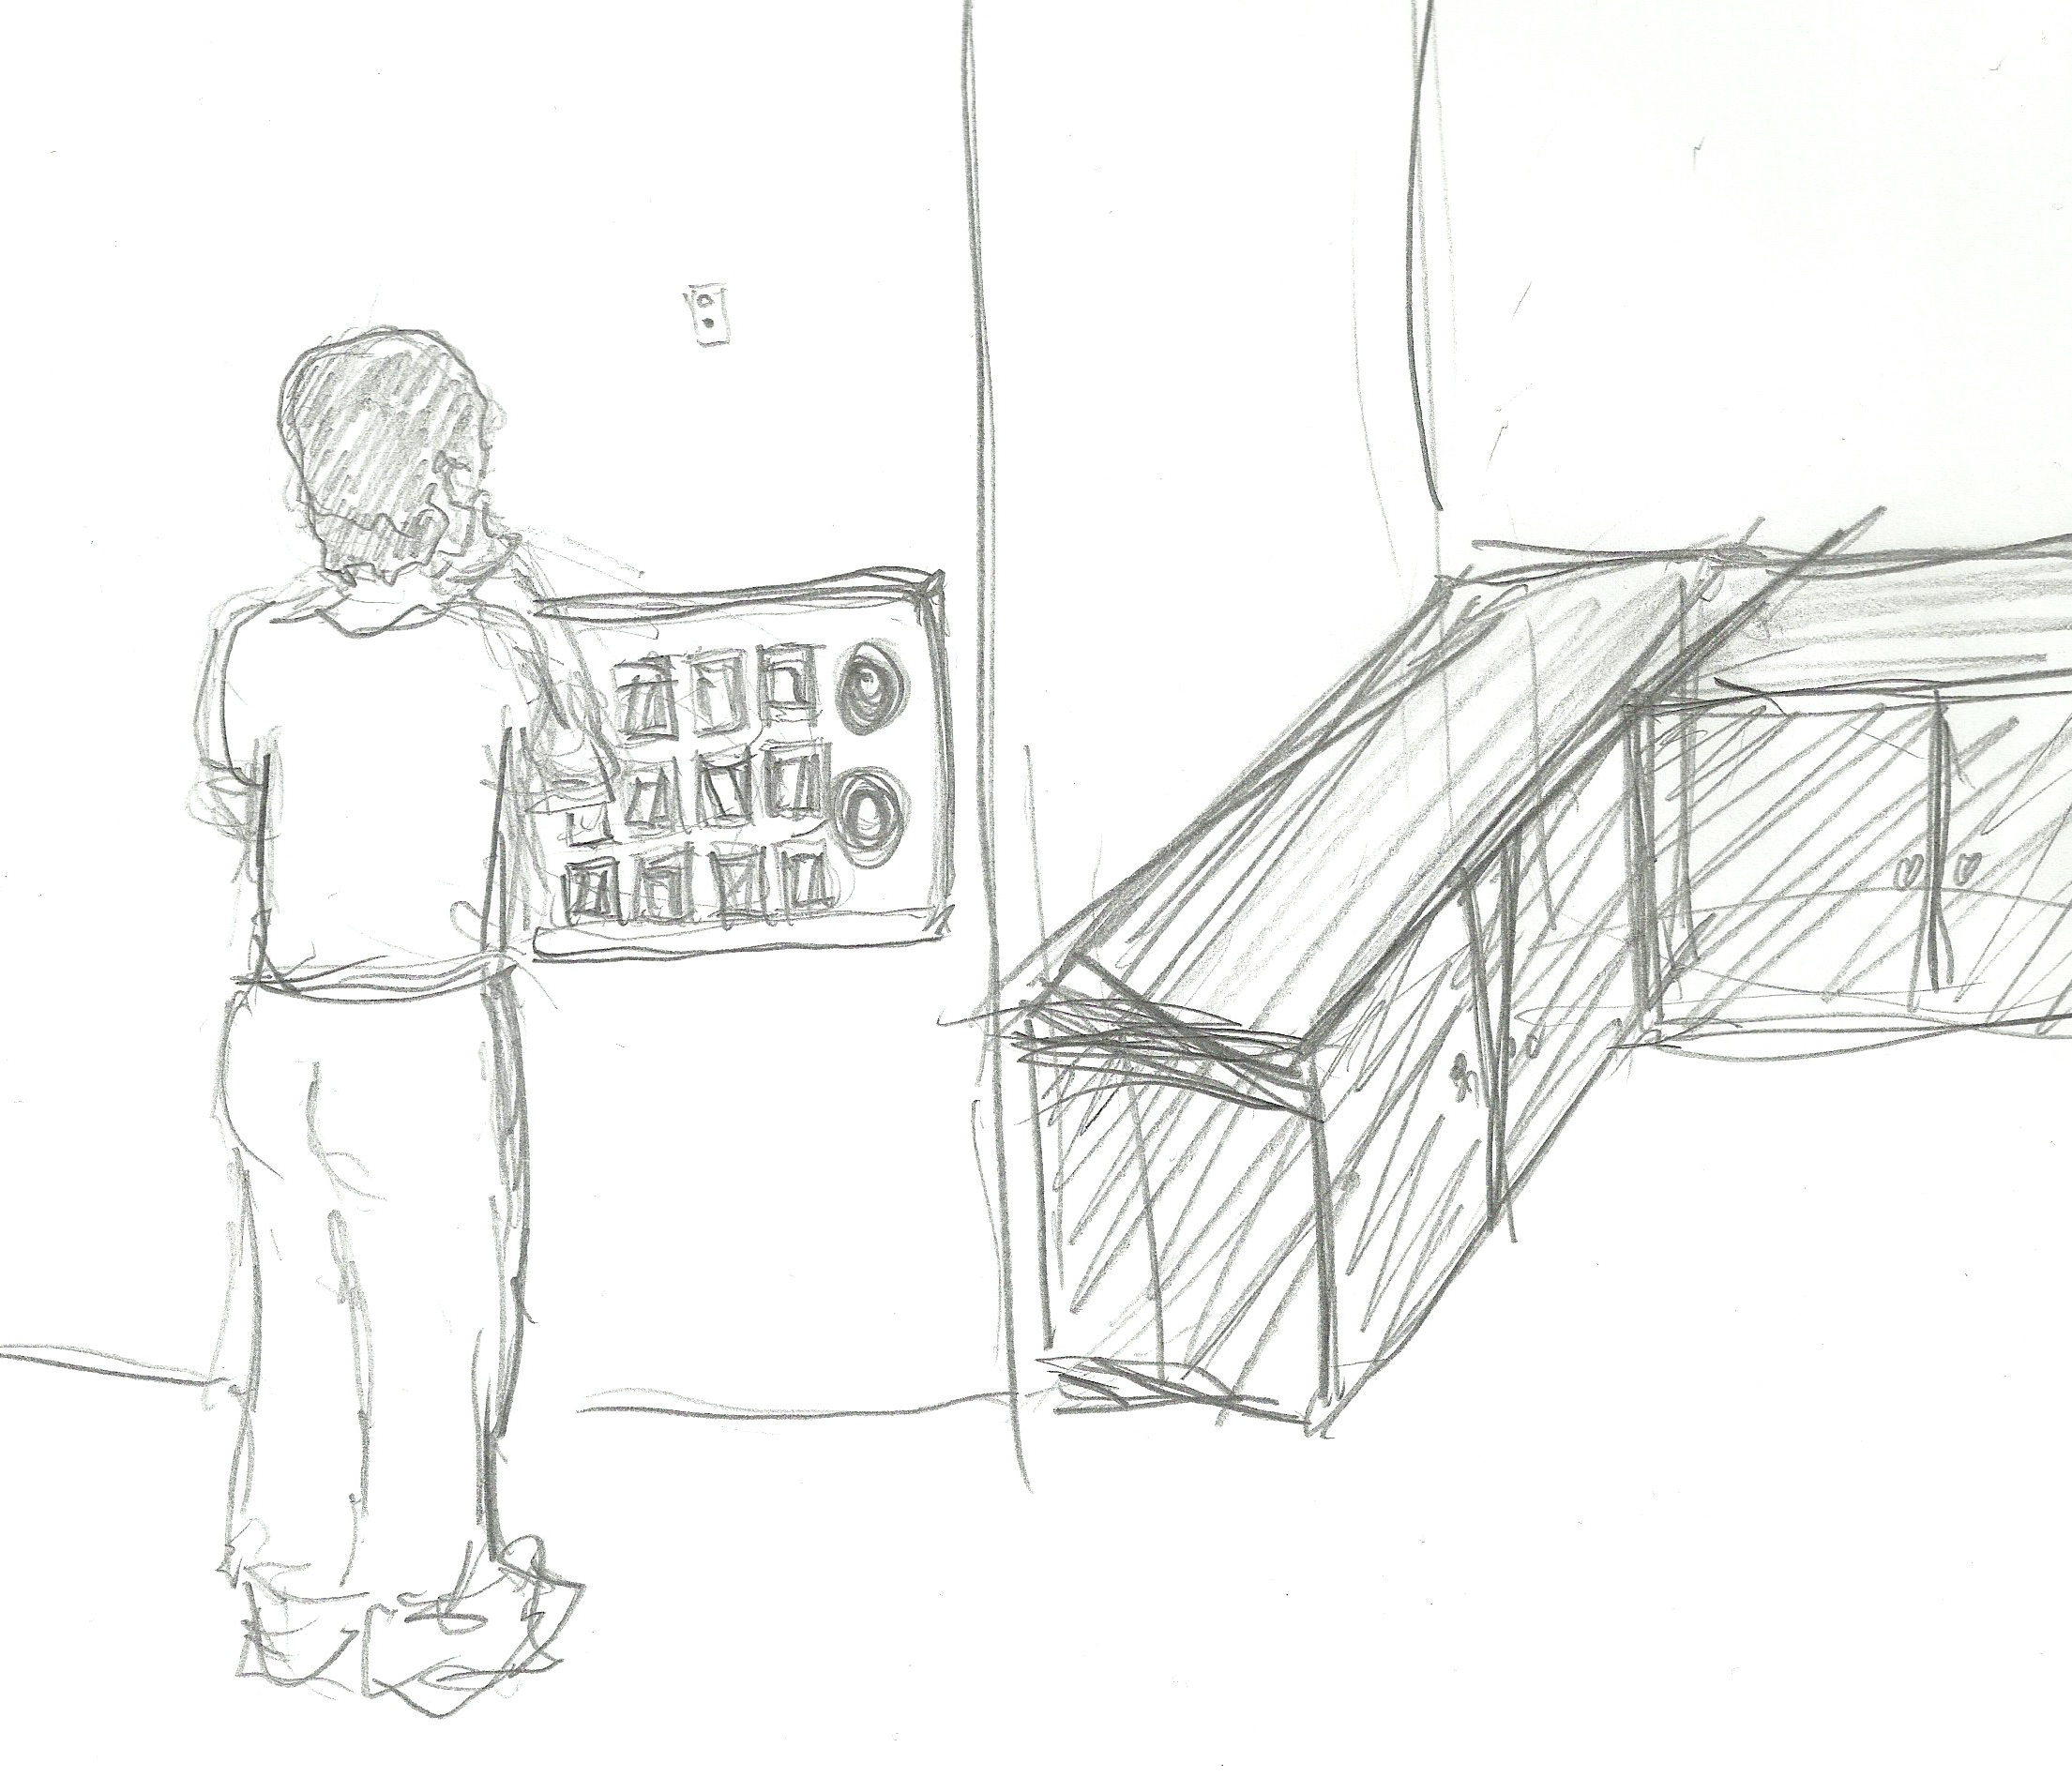
\includegraphics[scale=0.4]{fig/buttons}
\caption{Kommunikasjonssoner, gjenbrukt fra \citet{streitz05}. Displayet forandrer seg og tilbyr forskjellige interaksjonsmuligheter avhengig av hvilken sone brukeren befinner seg i.}
\label{commzones}
\end{figure}

Forskjellige interaksjonssoner beskrives av \citet{streitz05}. De omtaler interaksjonssonene omgivende, notifikasjon og interaksjon (figur \ref{commzones}). I den omgivende sonen kan brukeren oppfatte mønstere som vises på en vegg. Veggen sanser avstand til brukeren og viser mønstre ved å tenne et antall små, separate lyskilder. I notifikasjon vil personlige notifiseringsmønstre vises, og i interaksjon vil veggen vise spesielle mønstre og være interagerbar. Bruken av soner gir mulighet til å tilby forskjellige visninger og interaksjoner basert på avstand. Greenberg et al. omtaler fem målbare dimensjoner av \emph{proxemics}: \emph{Avstanden} mellom enheter og brukere virker naturlig, og passer godt inn med interaksjonssonene som er definert. \emph{Retning} gir et mål på vinkelen mellom enheter og brukere. Det finnes allerede enheter som gjør bruk av retning, for eksempel ved å skru seg av når folk ikke ser på dem. \emph{Bevegelse} omfatter forandring i distanse over tid. \emph{Identitet} beskriver en enhet i et gitt detaljnivå. \emph{Plassering} beskriver posisjonen til enheten, for eksempel i hvilket rom og hva konteksten rundt rommet er. \emph{Proxemics} kan i sin helhet være med på å tilby en mer naturlig interaksjon med enhetene våre og kan kanskje være det neste steget for utviklingen av interaksjonsapplikasjoner.

\subsubsection*{Gester}
En annen interaksjonsform det forskes på er gesturer. Dette er nok et forsøk på å tilby en mer naturlig interaksjon med datamaskinen. Kroppsspråket er tross alt en stor del av mellommenneskelig kommunikasjon, så hvorfor ikke forsøke å utvide det til kommunikasjon mellom menneske og maskin. \citet{homeos} omtaler en prosjektgruppe som utvidet HomeOS-systemet til å forstå gesturer, ved bruk av Kinect-kameraet. Det finnes mange prosjekter på nettet som har brukt Kinect til å skape systemer som forstår både gesturer og tale\footnote{Et godt dokumentert eksempelprosjekt som benytter Kinect's datasyn og talegjenkjenning: http://www.codeproject.com/Articles/715858/Home-Automation-with-Microsoft-Kinect-Point-Cloud, hentet des 2014.}. Ulempen med denne formen for gesturgjenkjenning er de samme som med sensorovervåking gjennom kameraer (kapittel 3.1): følelsen av overvåking og sikker håndtering av sensitive data. 

Det finnes andre, mindre påtrengende metoder for å detektere gesturer. Infrarøde gestur-sensorer kan tilby en kontaktløs interaksjon med det smarte hjemmet\footnote{SparkFun RGB and Gesture Sensor. Denne brikken kan måle lys, farge, avstand og gesturer: https://www.sparkfun.com/products/12787, hentet des 2014.}. Sensoren sender ut infrarøde signaler og mottar refleksjonen fra brukerens hånd. Mikrokontrolleren må så tolke disse verdiene til en gestur. Systemet kan dermed trenes med teknikker fra maskinlæring til å klassifisere og tolke forskjellige gesturer til å forskjellige kommandoer. Det infrarøde signalet reflekteres effektivt kun ut til en avstand på noen titalls centimeter. Dette blir dermed en mye mindre påtrengende metode enn bruk av video. Et bruksområde for gesturer kan være å be om det neste steget i en oppskrift, uten å måtte trykke på en touch-skjerm mens hendene er tilskitnet med mat. Det kan også være aktuelt å kombinere gesturer med en annen interaksjonsform, som tale. Et multimodalt brukergrensesnitt kan forbedre systemets nøyaktighet i tolkningen av kommandoene og avklare usikkerhet og misforståelser.

{\subsubsection{Hjemmet som en personlig assistent}
De fleste av oss har tilgang til en såkalt personlig assistent på smarttelefonen. På Android (og gjennom nettlesere) har man \emph{Google Now} og på iOS har man Apple's \emph{Siri}. Begge produktene er intelligente, personlige assistenter som tilbyr et brukergrensesnitt for naturlig språk hvor man kan få svar på spørsmål, anbefalinger og utførelser av handlinger gjennom web-tjenester. Begge tilpasser seg brukeren over tid og forsøker å levere individuelt tilpassede resultater.

I januar 2014 presenterte Intel et headset som i framtiden skal utfordre de personlige assistente fra Apple og Google, og de kaller det \emph{Jarvis}\footnote{http://www.theinquirer.net/inquirer/news/2325465/intels-jarvis-headset-will-take-on-apples-siri-and-google-glass-by-working-offline, hentet des 2014.}. Intel's fordel vil være at talegjenkjenningen utføres i headsettet, på den nye \emph{Edison-modulen}\footnote{http://www.intel.com/content/www/us/en/do-it-yourself/edison.html, hentet des 2014.}. Dermed fungerer den personlige assistenten selv når man ikke har kontakt med internettet. Når man kan unngå å sende forespørselen på en rundtur over nettet, for prosessering og analyse et annet sted, spares det mye tid og man unngår forsinkelsen som gjør dagens eksisterende systemer vanskelige å bruke. Science fiction inspirer ofte teknologisk utvikling og Intel's valg av navn er en klar referanse til datasystemet \emph{J.A.R.V.I.S.} fra \emph{Iron Man-filmene}\footnote{http://marvel-movies.wikia.com/wiki/J.A.R.V.I.S., hentet des 2014.}. Dette programmet styrer heltens smart hjem og kontrollerer alt der, som innemiljø og sikkerhet. Samtidig fungerer det som en personlig assistent og tilbyr hjelp med informasjonsgjenfinning og planlegging. Systemet interageres med gjennom touch-skjermer, talegjenkjenning, syntesert tale, holografi og robotikk. Så hvordan kan en slik personlig assistent som ikke bare tilbyr informasjon, men som selv utfører avanserte oppgaver, implementeres?

Mange webtjenester som folk flest bruker i dag, som kalendere, værkilder og trafikkdata, tilbyr også muligheten til å spørre kildene programmatisk gjennom API'er (\emph{application programming interfaces}. Dermed kan det smarte hjemmet kombinere sensordata fra huset med webtjenester. Basert på data fra kalendere, vær, trafikk og brukerens preferanser kan det smarte hjemmet for eksempel kalkulere at brukeren har tid til å gå til sitt første møte for dagen. Dersom brukeren svarer bekreftende på et slikt forslag kan systemet planlegge reiseruten til møtestedet og laste ned nødvendige kartdata til brukerens mobiltelefon. Dette er funksjonalitet som kan implementeres i dag. Et mer avansert scenario, der hjemmet gjør større, proaktive handlinger på brukerens vegne, og har muligheten for å hente informasjon fra informasjonskilder brukeren ikke kjenner til krever en annen teknologi. Dette er teknologi som eksisterer, men ennå ikke er utbredt. \citet{semantic01} legger grunnlaget for det neste steget i webbens evolusjon, en semantiske web. Dersom hjemmet for eksempel skal kunne kjøpe ønskede billetter på brukerens vegne trengs det en felles, vidspredt platform for kunnskapsrepresentasjon og en felles forståelse for beskrivelsen av og sammenhengene mellom informasjon. Først da kan systemer kommunisere seg i mellom uten menneskelig intervensjon på en trygg og sikker måte. En semantisk web foreslår \emph{Resource Description Framework (RDF)} for å representere kunnskap og avtalte ontologier for å beskrive informasjon og sammenhenger. At data er lagret i RDF gjør det enkelt å ta kontakt med mange forskjellige datakilder samtidig og lage kompliserte spørringer. Ontologiene gjør at det oppnås en felles forståelse for hvordan kunnskap henger sammen. Modellen som en helhet klargjør for å lage automatiserte agenter som kan kommunisere seg i mellom og utføre arbeid og transaksjoner som tidligere trengte sterk menneskelig innblanding, som å ta kontakt med en selgeragent hos en billettjeneste og bestille billetter på brukerens vegne.

\subsubsection*{Video -problemer med personvern}
Video gir potensialet for å realisere virkelig smarte systemer som kan motta kommandoer gjennom gesturer, forstå hjemmets tilstand, gjenkjenne beboerenes aktiviteter og kanskje til forstå kontekst. Video produserer store datamengder og dette gir en større teknisk utfordring med henhold til lagringsplass og datautvinning enn bruk av enklere sensorer. Heldigvis er det utviklet mange gode teknikker for å analysere bilder og desto mer tid som går desto større blir lagringskapasitetene våre.

Et eksempelprosjekt som blant annet gjør bruk av video er \emph{Placelab-prosjektet}, beskrevet av \citet{placelab05}. I sin studie gjorde de blant annet bruk av ni infrarøde kameraer, ni fargekameraer og atten mikrofoner spredd gjennom en leilighet. Ved bruk av bildebehandlingsalgortimer kunne de velge hvilke av datastrømmene som best fanget beboerens oppførsel til et gitt tidspunkt.

Baksiden av videomedaljen er beskyttelse av personvernet og brukerenes følelse av å opprettholde et privatliv i hjemmet. Intuitivt kan man forestille seg at de færreste brukere i utgangspunktet ønsker kameraer som filmer dem overalt i hjemmet. Selv dersom det kunne garanteres at informasjonen aldri forlot hjemmet, eller at den kun blir lagret i en kort tidsperiode, vil tilsynelatende konstant overvåking være noe mange vil sette et stort spørsmåltegn ved. I overvåkningssamfunnet i George Orwell's \emph{1984} har hver leilighet en skjerm med tilhørende kameraovervåking som kan se stort sett alt som foregår. I dette samfunnet har befolkningen over tid godtatt overvåkningen, i den tro at det er til deres eget beste. I vår verden ser ut til at folk flest godtar dagens nivå av overvåkning gjennom loggførte posisjonsdata fra smarttelefoner, søkeord og forflytninger med fly og bil. Men introduksjonen av videokameraer i stuene vil kanskje oppleves som for mye, selv hvis informasjonen kun holdes og brukes lokalt.

%%=========================================
\subsubsection*{Problemformulering}
asd

%%=========================================
\subsection{Mål}
Basert på dette arbeidet ønsker jeg å jobbe videre med en masteroppgave som omhandler brukergrensesnitt i forbindelse med smarte hjem. Spesielt vil det være spennende å utforske alternativer til touch-skjermer og laptoper for å kommunisere med hjemmet. Basert på resultatene fra brukerstudiene og Rogers argumenter presentert i kapittel seks er jeg overbevist om at vi ikke ønsker et proaktivt hjem hvor brukerene lener seg tilbake og lar omgivelsene ta seg av alt. Jeg tror vi ønsker å bli engasjert og at spennende og utfordrende brukergrensesnitt kan være med på å skape en ny renessanse for interaksjonen med datamaskinen.

Våren 2015 vil jeg jobbe med bruken av gesturer for å interagere med et smart hjem. Dette kan bli i en multimodal setting der man også gjør bruk av touch-skjermer og/eller tale. Oppgaven peker mot at mange mennesker ikke ønsker kameraer i hjemmene sine. Da passer i steden for de infrarøde gestur-sensorer presentert i kapittel seks godt. Arbeidet kan omhandle faktiske brukere og utforske om gesturer er en verdifull måte å interagere på. En annen tilnærming kan være å bruke maskinlæring for å få systemet til å lære å tolke ulike gesturer gjennom klassifisering. Et tredje alternativ er å kombinere gesturer med annen input og se om multimodal interaksjon kan forbedre systemets nøyaktighet og avklare misforståelser.
Hovedmålene for dette prosjektet er å
\begin{enumerate}
\item Utforske bruken av enkle gestesensorer kombinert med talegjenkjenning som en effektiv og naturlig interaksjon med hjemmet.
\item Utforske kontekstdrevne brukergrensesnitt.
\end{enumerate}

%%=========================================
\subsection{Begrensninger}
asd

%%=========================================
\subsection{Rapportens struktur}
Dette introduksjonskapitellet etterfølges av fire interaksjonsprosjekter, samt et avsluttende kapittel. 
%%=========================================
\section{Gestegjenkjennelse med fotodioder}
%%=========================================
\subsection{Introduksjon}
Når hjemmet ditt om noen år tilbyr kontroll over ikke bare lys og temperatur, men garasjeporter, persienner, tv'er, radioer, låsene på døra og statusen til kjøkkenapparater, kan det være en utfordring å tilby gode interaksjonsmetoder. Den vanlige måten er enten å la kontrollknappene bo ved apparatet, samle de i et panel på veggen, eller samle de i en fjernkontroll eller app. Med et økende antall styrbare apparater blir det upraktisk å kun ha kontroll dersom man fysisk befinner seg ved apparatet. Å tilby kontroll i en fjernkontroll eller app kan være praktisk, men hva hvis denne mobile enheten blir gjenglemt et sted? En fjernkontroll eller app må også designes svært godt for å ikke skape forvirring med et vanskelig brukergrensesnitt. Spesielt en fjernkontroll vil gi uinnvidde brukere, som gjester eller beboere av et nyanskaffet system, svært store vanskeligheter. Så kanskje vi ønsker å ha et sted i rommet der kontrollen samles. Vel, et panel med knapper er ikke bare stygt, men det er vanskelig å vite hvilke knapper som hører til hvilken funksjonalitet (se figur \ref{fig:panel}). Hva hvis vi i stedet kunne tilby et eller flere punkter på veggen på størrelse med et knappenålshode som forstår en rekke enkle, men ulike gester? 
 
Denne ideén om å kontrollere ved hjelp av gester er ikke ny {\color{red} refererfef}. Tilnærmingen i disse prosjektene er kameraer som måler farger og dybde samt avanserte algortimer for datasyn. Sammen kan disse prosessere informasjonen og danne grunnlaget for et system som kan gjenkjenne kompliserte gester. Vel, bruken av kameraer har visse problemer i hjemmescenariet. {\color{red} Ref og ref} har vist at brukere har sterke motsetninger mot overvåking i sitt eget hjem. Selv dersom det kan garanteres at dataene fra kameraene holdes lokalt kan følelsen av at personvernet er utsatt være nok til at brukerene vil holde seg unna. Vi ønsker en alternativ måte å interagere med funksjonaliteten i hjemmet. Den skal være naturlig, effektiv og må garantere et vern av personvern og privatliv.

\begin{figure}
\centering
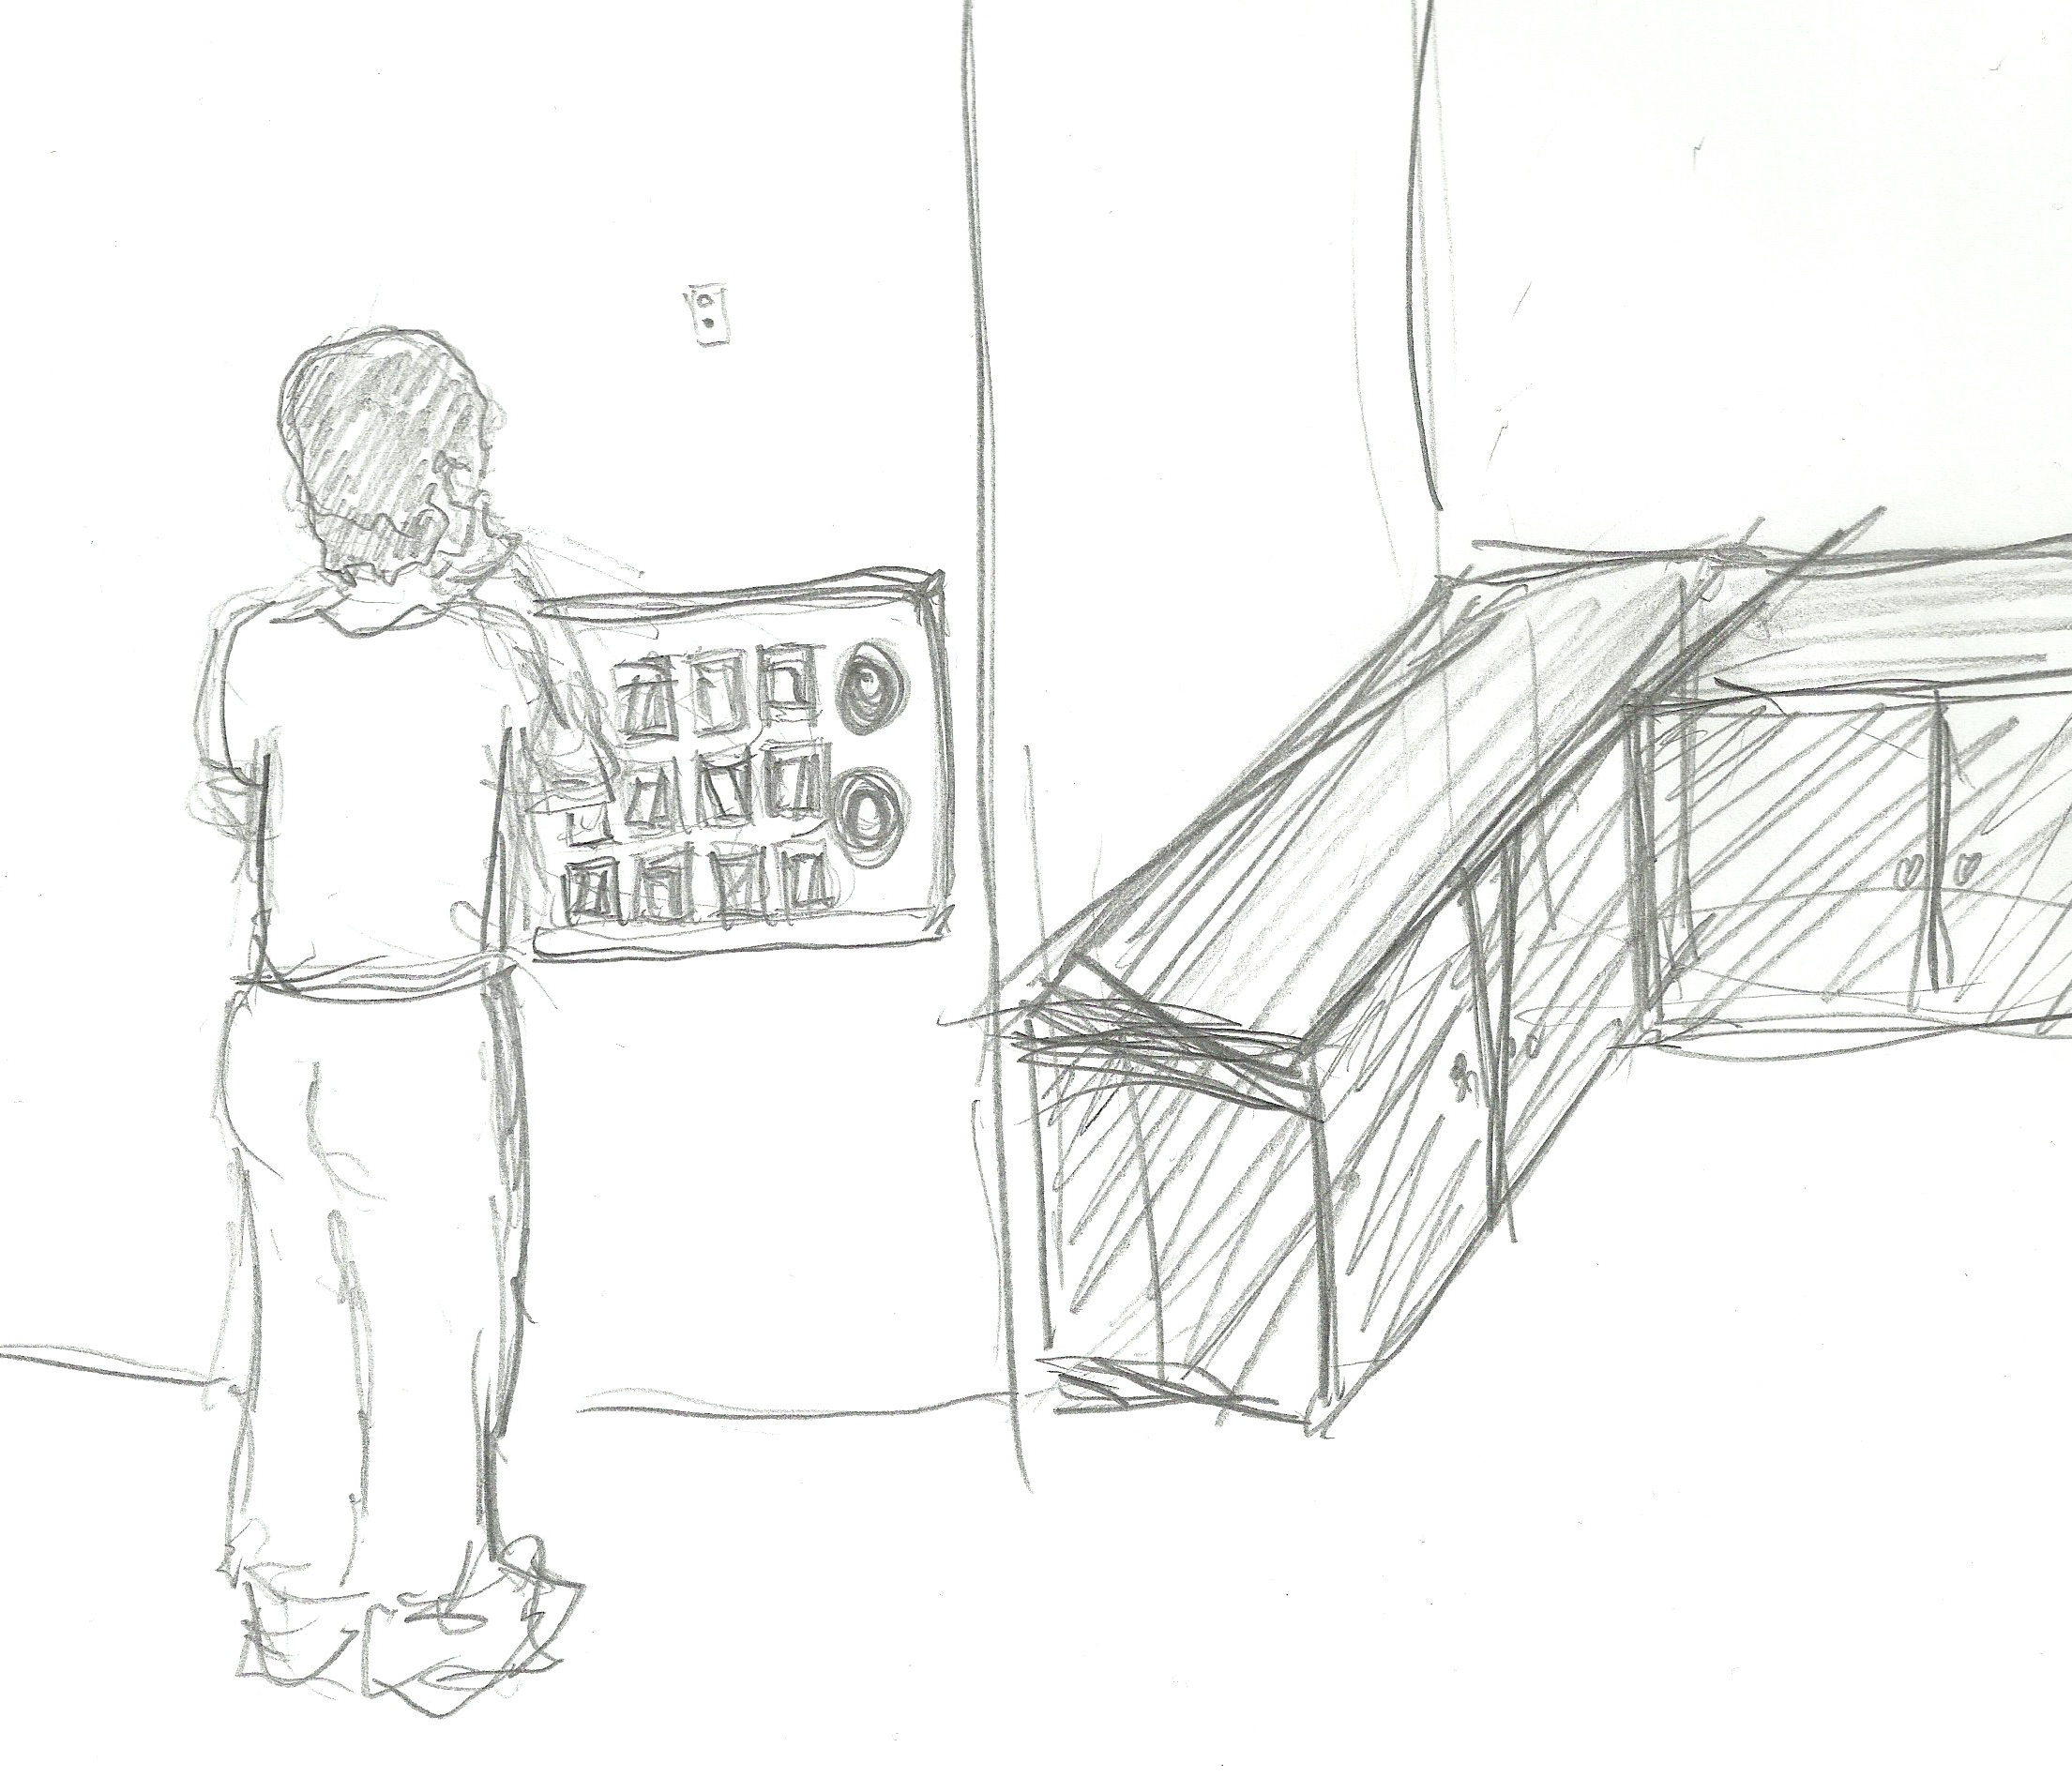
\includegraphics[scale=0.1]{fig/buttons}
\caption{En vegg med knapper skaper forvirring.}
\label{fig:panel}
\end{figure}

Dette kapittelet har følgende bidrag:
\begin{itemize}
\item Jeg argumenterer for at en gestesensor i form av enkle fotodioder er et tilstrekkelig medium for enkel brukerinteraksjon (\ref{ch:2.minide}).
\item Jeg viser at maskinlæring kan benyttes for å lære et system å forstå enkle gester og viser at dette er et alternativ til å eksplisitt programmere forståelse (\ref{ch:2.resultater}).
\item Jeg viser at det holder med et titalls treningseksempler fra hver gest for å oppnå gode resultater med lineære modeller og at det med 50 eksempler oppnås en suksessrate på 96\% (\ref{ch:2.resultater}).
\end{itemize}

\subsection{Interaksjon gjennom gester}
\label{ch:2.minide}
Dette avsnittet presenterer hovedideén for dette kapitellet. 
Dersom man ønsker å tilby styringsmuligheter på en eller flere vegger i et hus kan enkle gestesensorer benyttes i steden for et panel av knapper og dimmere. Selve sensoren er på størrelse med et knappenålshode og vi kan dermed forestille oss at designere kan komme opp med produktimplementasjoner som enten forsvinner inn i hjemmiljøet eller synes tydelig, men er praktisk og estetisk veldesignet. Sensoren merker at en hånd eller et annet objekt befinner seg foran den ved å sende ut et svakt infrarødt signal som reflekteres og detekteres dersom signalet er sterkt nok når det returnerer. Dette vil bare skje dersom objektet er opptil 20 cm unna sensoren. Dette betyr at gester kun forstås dersom de utføres rett foran sensoren. I motsetning til gesteforståelse gjennom bruk av kameraer er dette altså en langt mindre påtrengende måte å "lytte" etter input fra brukerne. Brukere kan være sikre på at de hverken overvåkes eller at personvernet deres på noen måte brytes. En slik gestesensor fungerer rett og slett kun som en multifunksjonell knapp.

\begin{wrapfigure}{r}{0.4\textwidth}
    \vspace{-20pt}
  \begin{center}
    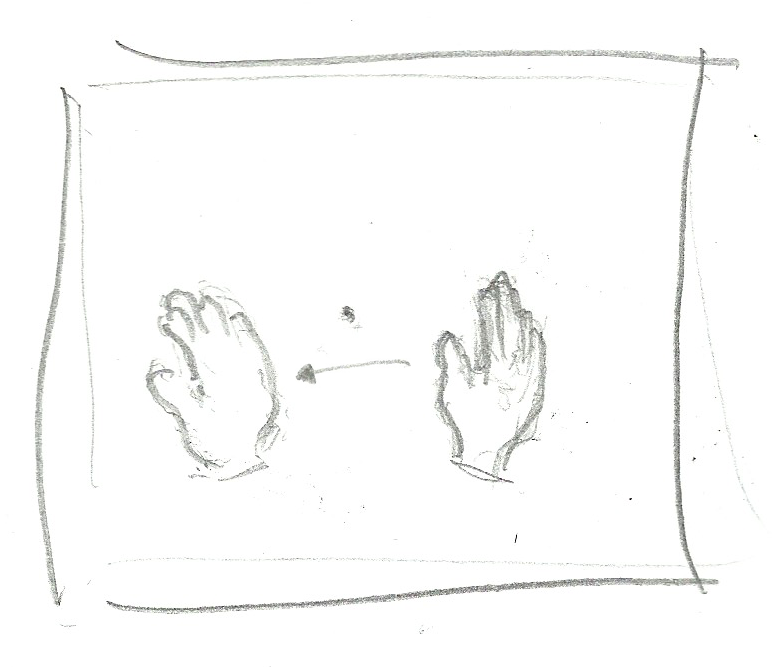
\includegraphics[width=0.35\textwidth]{fig/swipe-l-r}
  \end{center}
  \vspace{-20pt}
  \caption{Illustrasjon av en typisk gest.}
  \label{fig:gest}
  \vspace{-7pt}
\end{wrapfigure}

Figur \ref{fig:gest} viser en typisk gest der brukeren sveiper hånda foran sensoren som befinner seg på veggen. Vi kan forestille oss at denne sveipende bevegelsen foran denne sensoren betyr å skru av lyset i rommet sensoren befinner seg i. Men kanskje gesten betyr å skru på radioen, lukke gardinene eller starte kaffemaskinen. Det er ingen begrensning på hva en enkelt gest aktiverer i form av funksjonalitet.

Når en gest utføres må enten rådataene fra sensoren eller en forståelse av dataene sendes til en maskin som har ansvaret for å styre apparatene i hjemmet. Sensoren må være knyttet til en mikrokontroller eller tilsvarende som har ansvaret for å sende dataene videre. Dette kan enten være gjennom kabel eller trådløst. Det er mulig å programmere en mikrokontroller til å skille mellom sensordataene og forstå seks ulike gester {\color{red} ref}. Dette er i seg selv bra og betyr at en enkelt sensor kan fungere som en multifunksjonell knapp med minimum seks forskjellige kommandoer. Hvis man også utnytter at kombinasjonen av flere gester etter hverandre kan bety egne kommandoer er styringsmulighetene mange. Det finnes et alternativ til å programmere inn hva de ulike dataene skal tolkes som. Alternativet er å sende rådataene til en kraftigere maskin som kan benytte den spennende teknikken kjent som maskinlæring til å forstå enda flere ulike gester, med god sannsynlighet for suksess.

Maskinlæring handler om å la maskinen lære fra data. Dette kan enten være et forsøk på å finne ukjente sammenhenger i dataene den mates med eller det kan være å lære seg sammenhenger mellom dataeksempler og etiketter/klasser. Det er dette sistnevnte scenariet vi er interessert i. Vi kan mate maskinen med data fra en gest og samtidig gi informasjon om at dataene maskinen akkurat fikk betyr "sveip til høyre". Dermed kan maskinen danne en knytning mellom dataene som kom inn da vi sveipet til høyre og etiketten "sveip til høyre". Med tilstrekkelig treningseksempler fra de ulike gestene skal maskinen kunne lære seg forskjellene mellom de ulike gestene. Dermed vil den være i stand til å gjette riktig på hvilken gest vi utfører ved en senere anledning. Prototypen jeg har utviklet er trent med 50 ulike dataeksempler på hver av de 10 ulike gestene.

\begin{figure}[h]
\begin{subfigure}{0.23\textwidth}
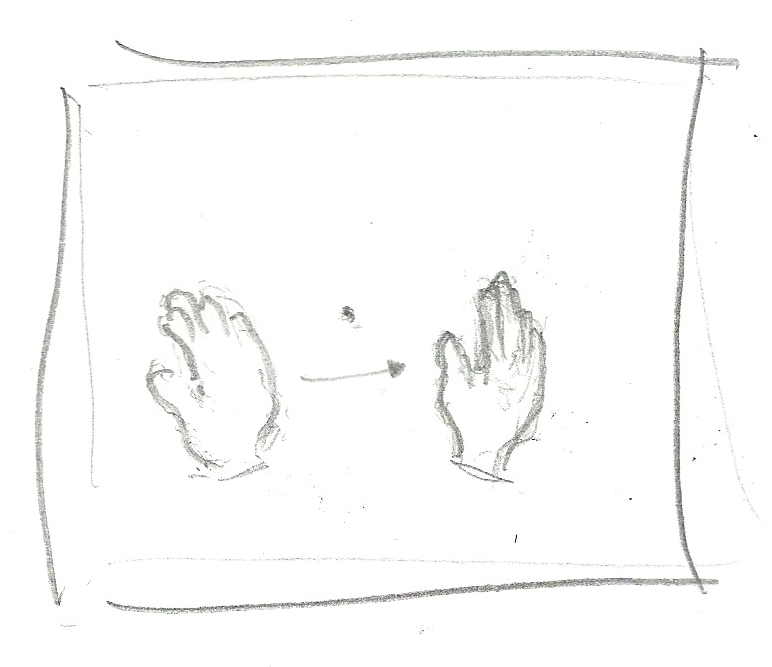
\includegraphics[width=3cm, height=3cm]{fig/swipe-r-l}
\caption{Sveip til høyre.}
\label{fig:sveip-}
\end{subfigure} 
\begin{subfigure}{0.23\textwidth}
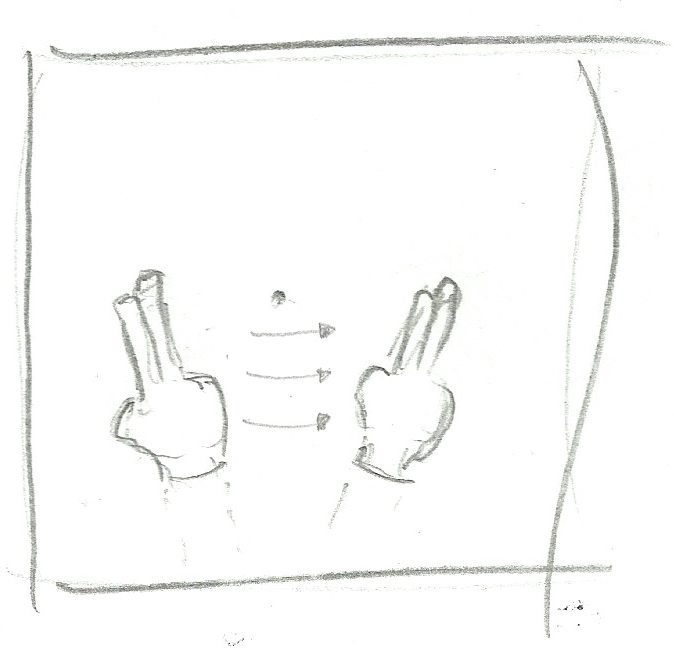
\includegraphics[width=3cm, height=3cm]{fig/flick-l-r} 
\caption{Flikk til høyre.}
\label{fig:flikk-h}
\end{subfigure}
\begin{subfigure}{0.23\textwidth}
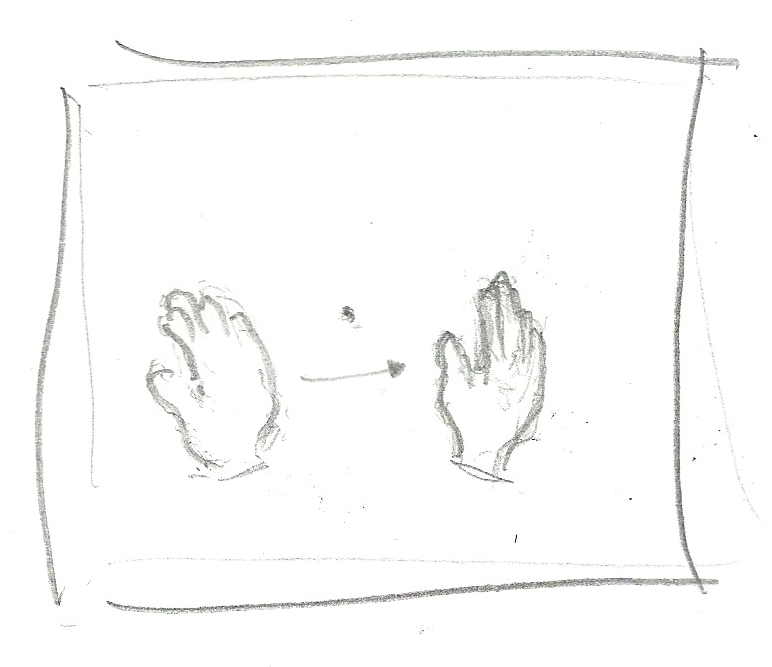
\includegraphics[width=3cm, height=3cm]{fig/swipe-r-l}
\caption{Sveip til venstre.}
\label{fig:sveip-v}
\end{subfigure} 
\begin{subfigure}{0.23\textwidth}
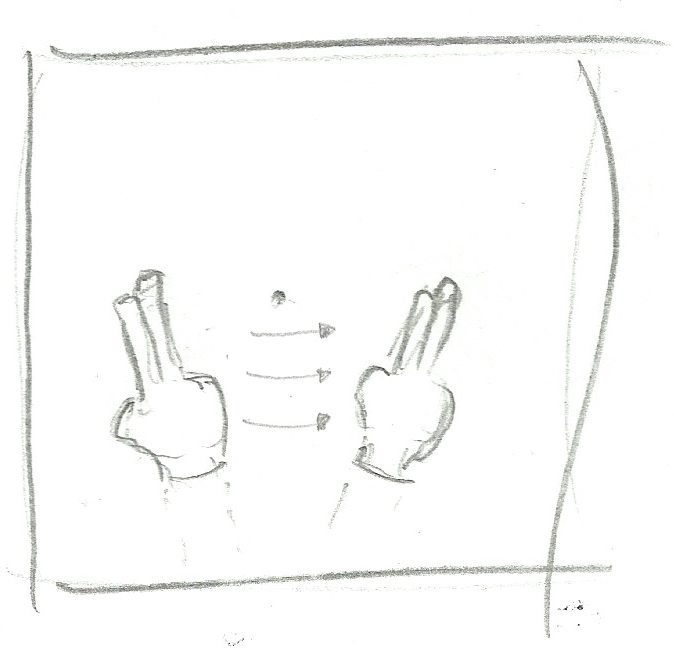
\includegraphics[width=3cm, height=3cm]{fig/flick-l-r}
\caption{Flikk til venstre.}
\label{fig:flikk-v}
\end{subfigure}
\begin{subfigure}{0.23\textwidth}
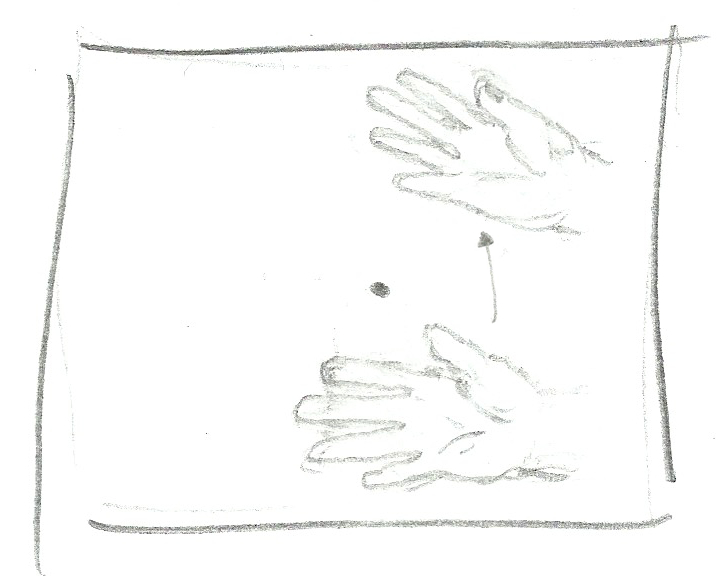
\includegraphics[width=3cm, height=3cm]{fig/swipe-d-u}
\caption{Sveip opp.}
\label{fig:sveip-opp}
\end{subfigure}
\begin{subfigure}{0.23\textwidth}
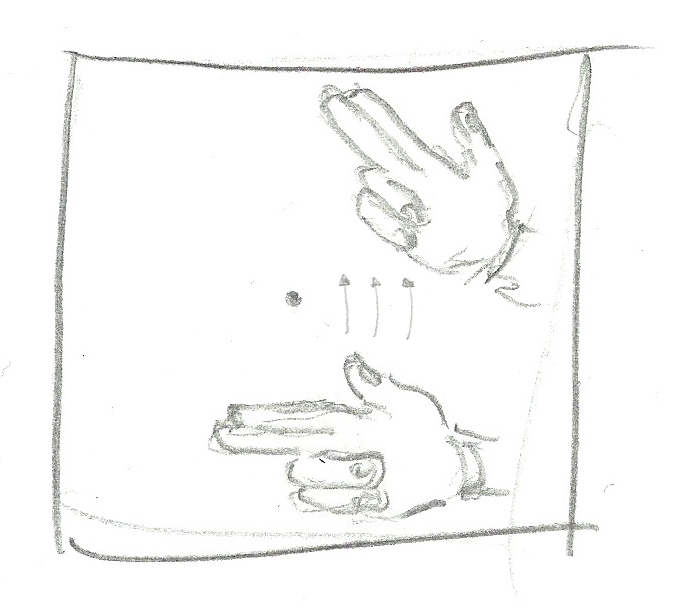
\includegraphics[width=3cm, height=3cm]{fig/flick-d-u}
\caption{Flikk opp.}
\label{fig:flikk-opp}
\end{subfigure}
\begin{subfigure}{0.23\textwidth}
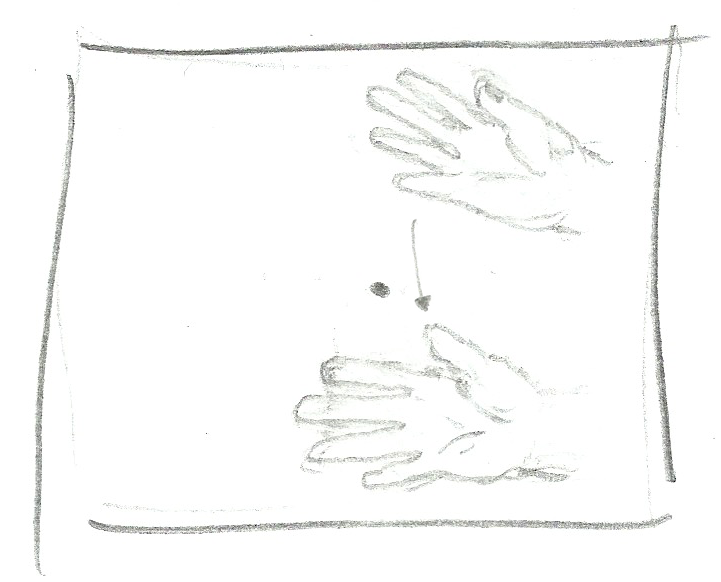
\includegraphics[width=3cm, height=3cm]{fig/swipe-u-d}
\caption{Sveip ned.}
\label{fig:sveip-ned}
\end{subfigure}
\begin{subfigure}{0.23\textwidth}
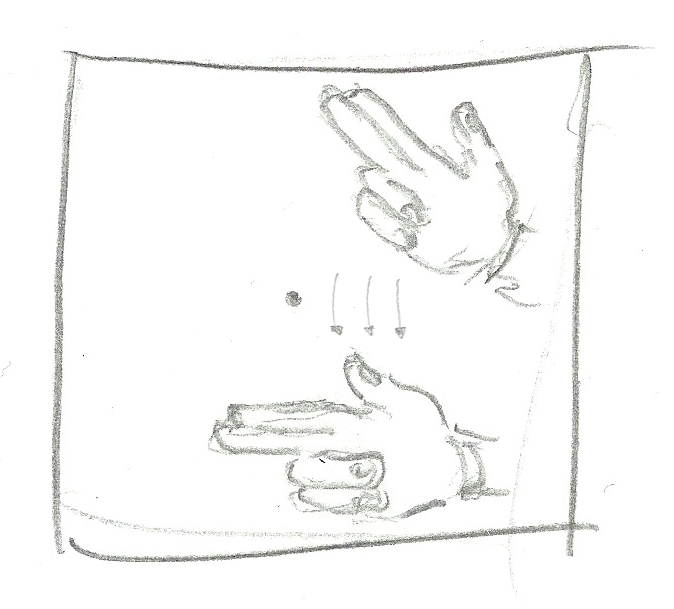
\includegraphics[width=3cm, height=3cm]{fig/flick-u-d}
\caption{Flikk ned.}
\label{fig:flikk-ned}
\end{subfigure}
\begin{subfigure}{0.25\textwidth}
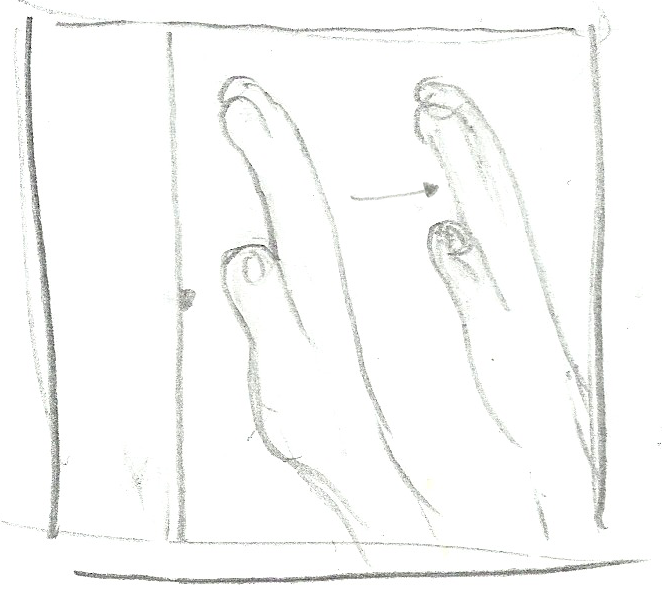
\includegraphics[width=3cm, height=3cm]{fig/near-far}
\caption{Nær - fjern.}
\label{fig:n-f}
\end{subfigure}
\begin{subfigure}{0.23\textwidth}
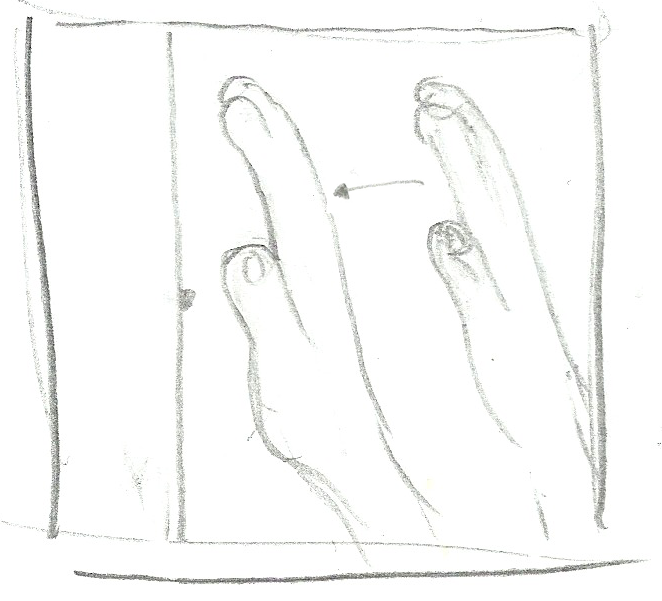
\includegraphics[width=3cm, height=3cm]{fig/far-near}
\caption{Fjern - nær.}
\label{fig:f-n}
\end{subfigure}
\caption{Illustrasjon av de ulike gestene.}
\label{fig:gester}
\end{figure}

\subsection{Detaljer}
\subsubsection{Hardware}
Sensoren som benyttes i denne prototypen er APDS-9960 fra Avago Technologies. Sensoren tilbyr måling av lys og farge, oppdagelse av nærhet og gestegjenkjennelse\footnote{Kapittel 4 utforsker bruksområder for funksjonaliteten rundt lys, farge og nærhet.}. Innpakningen er svært liten på kun 3.94 * 2.36 * 1.35 mm. Selve gestesensoren består av fire fotodioder som merker et reflektert infrarødt signal utsendt fra en LED. Fotodiodene er vinklet litt forskjellig slik at de plukker opp refleksjoner på litt forskjellige steder. Den benytter resultater fra nærhetsdetektoren for å automatisk aktiveres når et objekt er innen rekkevidde. I tilegg brukes måling av lys for å tilpasse de infrarøde målingene til lysnivået i omgivelsene. Dataene dannes som 32-bit datasett og kommuniseres over I2C-protokollen til en mikrokontroller. Gestesensoren kan selv håndtere forståelse av gester som passerer opp, ned, mot venstre eller mot høyre over sensoren, men denne funksjonaliteten tar vi ikke i bruk her {\color{red} ref apds9960-dokumentasjonen.}.

Prototypen er utviklet med Sparkfun's innpakning av APDS9960-sensoren\footnote{https://www.sparkfun.com/products/12787}. Denne brettet gjør APDS9960-sensoren tilgjengelig for enkel prototyping ved å bryte ut ulike pinner. {\color{red} bilde av sparkfun-brikken som peker ut hvilken del som er apds9960.} I tillegg har de gjort tilgjengelig programvare til Arduino-plattformen\footnote{http://www.arduino.cc/} så utviklere kommer raskt i gang. De ulike programmene som kan lastes opp til en Arduino gir tilgang til de forskjellige funksjonalitetene hos APDS-9960-brikken.

\subsubsection{Dataprosessering}
Seriell data sendes fra mikrokontrolleren til datamaskinen som lytter på riktig port. Sensoren sender data så lenge ir-signalet reflekteres. Dette betyr at en gest som tar lengre tid skaper mer data. Et rolig sveip over sensoren med hele hånda kan skape 100-200 datapunkter. Et raskt flikk med to fingre skaper 16-32 datapunkter. En gest som involverer å holde hånda foran sensoren i et sekund eller mer skaper flere hundre datapunkter. For å benytte de planlagte klassifiseringsteknikkene må hvert av treningseksemplene må ha like mange egenskaper.

Det finnes ulike metoder for å løse dette problemet. En av de er å bestemme et øvre antall maksimale egenskaper som skal tas med. Inputeksempler som ikke har tilstrekkelig med egenskaper blir paddet med 0-verdier. Å sette en maksgrense på egenskaper kan føre til at man mister viktig data fra gester som tar lengre tid å utføre. For et inputeksempel fra en rask gest vil mange egenskaper være 0. Dette kan påvirke effektiviteten til læringsalgoritmen. Et annet alternativ er å velge et fast antall egenskaper vært inputeksempel skal ha og så knytte inputeksempelet til denne egenskapervektoren. Dersom input har få datapunkter blir egenskapvektoren sparsom med data spredt jevnt utover og med 0-verdier i mellom. Dersom input har mye data vil hver egenskap i egenskapsvektoren være et gjennomsnitt av en viss mengde datapunkter.

Jeg valgte å lage vektorer med 128 egenskaper. Dette tallet ble valgt basert på antall datapunkter som genereres ved ulike aktuelle gester. 128 egenskaper er nok til å gi tilstrekkelig detaljer selv ved gester som tar noe lengre tid og samtidig ikke så mange at raske gester skaper for sparsomme resultater. Egenskapsvektoren normaliseres ved å knytte de mulige sensorverdiene 0-255 til 0-1.0. Å illustrere dannelsen av vektorere med 128 egenskaper blir tungvint så i figur \ref{fig:data} har jeg illustrert prosessen med mindre data. I \ref{fig:few} består inputvektoren av to datapunkter. Vi ønsker en egenskapsvektor med størrelse fire. Dette oppnås ved å spre inputdataene jevnt i egenskapsvektoren og normalisere verdiene. \ref{fig:many} viser det motsatte tilfellet, der inputvektoren er for stor. For å representere dataene i en mindre egenskapsvektor blir det tatt gjennomsnittsverdier som deretter normaliseres. 

\begin{figure}[h]
\centering
\begin{subfigure}{0.23\textwidth}
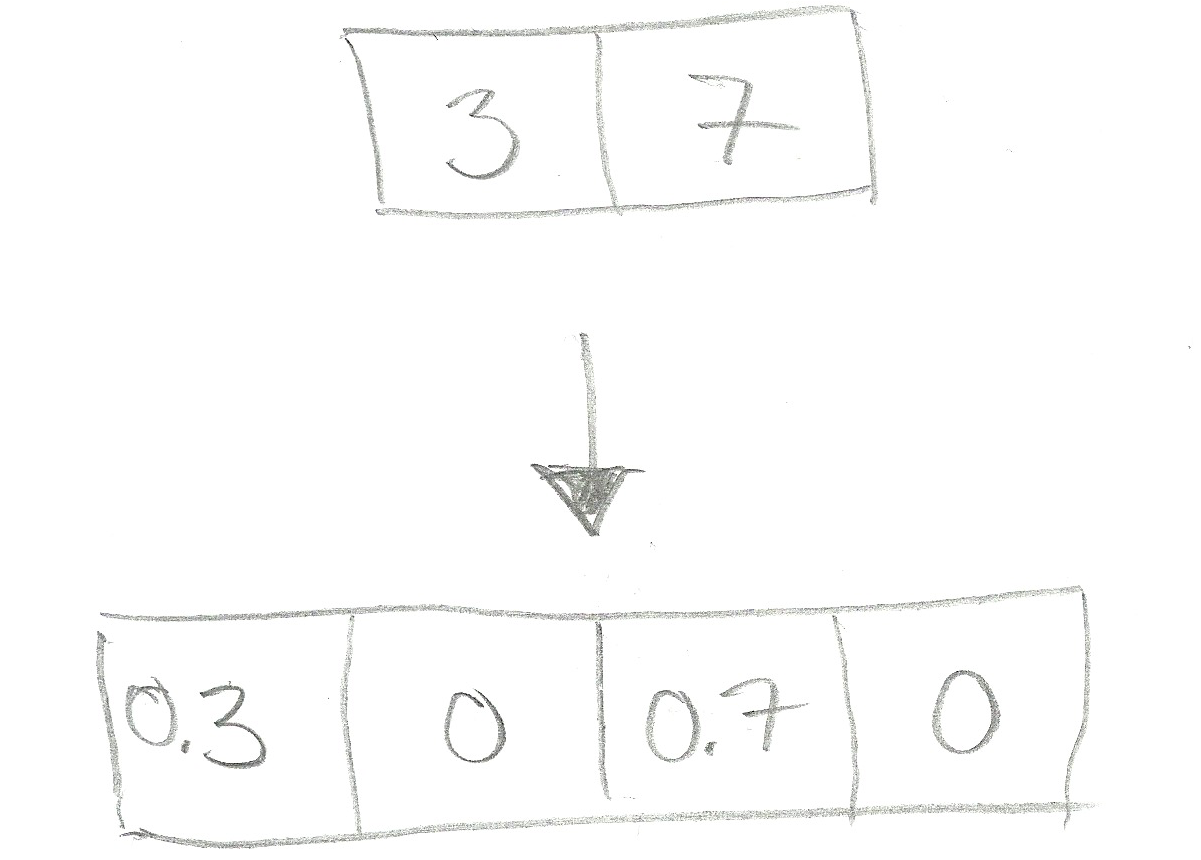
\includegraphics[width=3cm, height=3cm]{fig/few-to-many}
\caption{Sveip til høyre.}
\label{fig:few}
\end{subfigure}
\begin{subfigure}{0.23\textwidth}
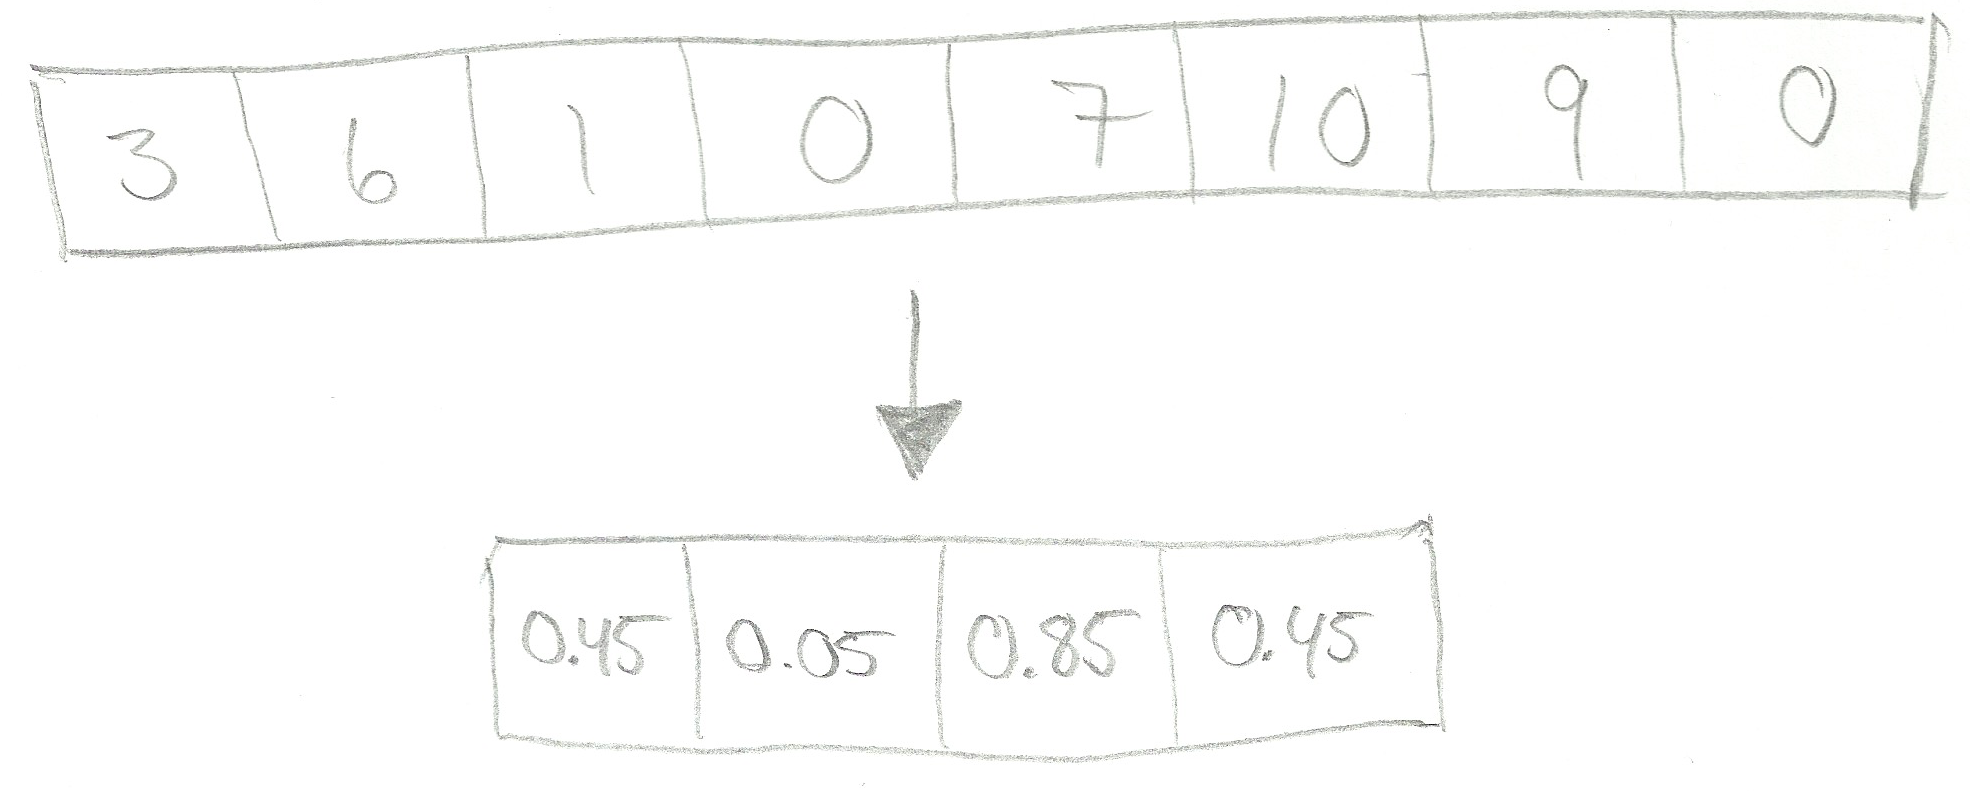
\includegraphics[width=3cm, height=3cm]{fig/many-to-few}
\caption{Sveip til høyre.}
\label{fig:many}
\end{subfigure}
\caption{Illustrasjon av dannelsen av en egenskapsvektorer.}
\label{fig:data}
\end{figure}

{\color{red} ref process-data.py/trim-data}

\subsubsection{Maskinlæring: Klassifisering}
La oss begynne med en definisjon på maskinlæring fra Arthur Samuel (1959): "Maskinlæring gir datamaskiner evnen til å lære uten å bli eksplisitt programmert."

Denne definisjonen er over 50 år gammel, men den fanger hva vi er ute etter. Vi er interessert i å få datamaskinene til å lære å gjøre nyttige ting uten å behøve å fortelle dem eksplisitt hvordan hver enkelt oppgave skal utføres. Dette er nødvendig da det med mye og kompleks data raskt blir umulig å beskrive alle deloppgavene som må utføres.

Alle maskinlæringsproblemer kan konseptualiseres som å finne en funksjon som knytter input til output. Målet kan være å tilnærme en enkel matematisk funksjon, det kan være å spå aksjekursen basert på historisk data eller det kan være å gi sannsynligheten for et en epost er spam, basert på innholdet. Man tar erfaring i form av empirisk data og kjører det gjennom en algoritme som automatisk skaper en funksjon som forsøker å dekke denne kunnskapen.

I dette prosjektet skal dataene en gest danner knyttes til navnet på en gest. Dette er en form for maskinlæring kalt overvåket læring og målet er korrekt klassifisering av dataene. Læringen er overvåket fordi vi bidrar med informasjon om hvilke klasser som hører til hvilke data i treningseksemplene. Framgangsmåten er å mate maskinen med mange treningseksempler på denne koblingen mellom data og gest og håpe at maskinen finner en matematisk funksjon som tilnærmer denne sammenhengen godt.

Dataene vi jobber med i dette prosjektet har 128 egenskaper og 50 treningseksempler av hver klasse. Dette er relativt mange egenskaper og få treningseksempler. Basert på disse karakteristikkene er det sannsynlig at enkle, lineære modeller vil gi de beste resultatene. Mer avanserte klassifiseringsteknikker, som for eksempel nevrale nettverk, kan i teorien tilnærme enhver funksjon, men de trenger langt flere treningseksempler for å finne de sanne sammenhengene mellom datapunktene.

Vi mater et treningssett av datapunkter til en valgt læringsalgoritme. Algoritmen danner seg en hypotese om hva slags modell som best beskriver dataene. Denne hypotesen kan så benyttes til å gjøre gjetninger på nye datapunkter. Hypotesen avhenger av egenskapene/variablene/kvalitetene {\color{red} hvilket ord er best?} i datapunktene. I en lineær modell er hypotesen en funksjon av egenskapene $x$ i treningsdataene, der hver egenskap blir vektet av $\theta$-verdier:

\begin{equation}
h_\theta(x) = \theta_0 + \theta_1x_1 + \theta_2x_2 + ... + \theta_nx_n
\label{eq:hypotese-lin}
\end{equation}

I dette prosjektet har vært datapunkt $n = 128$ egenskaper. La oss modellere $x$ til å være en vektor av disse egenskapene: 
\[
x =
\begin{bmatrix}
x_0 \\
x_1 \\
x_2 \\
.. \\
x_n
\end{bmatrix}
\in R^{n+1},
\]
Vi lar $\theta$ være en tilsvarende vektor: 
\[
\theta =
\begin{bmatrix}
\theta_0 \\
\theta_1 \\
\theta_2 \\
.. \\
\theta_n
\end{bmatrix}
\in R^{n+1}
\]

Dersom vi nå tar den transponerte av $\theta$ og lar \(x_0 = 1\), kan vi i stedet for (\ref{eq:hypotese-lin}) skrive hypotesen kompakt som:
\begin{equation}
h_\theta(x) = \theta^{T}x
\label{eq:hypotese-kompakt}
\end{equation}

En vellykket hypotese vekter $\theta$-verdiene godt for å maksimere ytelsen på algoritmen. Dette er det samme som å finne hvilke egenskaper i dataene som er de viktigste for å representere likheter/ulikheter (?). Så hvordan velger man disse $\theta$-verdiene? Vi ønsker $\theta$-verdier slik at hypotesen \(h_\theta(x)\) er nære klassen $y$ for treningseksemplene \((x,y)\) som knytter data til klasse. Dersom vi antar at hypotesen er en lineær funksjon og at dataene kun har to egenskaper kan vi plotte hypotesen som en linje gjennom datapunktene. For hvert nye treningseksempel vil $\theta$-verdiene justeres og linjen vil tilpasses og følge datapunktene som angir en av klassene bedre. Etter at funksjonen er trent på en rekke treningseksempler vil linjen forhåpentligvis danne et så klart skille som mulig mellom datapunktene som utgir de to klassene {\color{red} graf?}.

Det er vanskelig for oss å forestille oss en separator som opererer i mer enn tre dimensjoner. Heldigvis kommer matematikken til vår hjelp da den ikke bryr seg om våre visuelle begrensninger og allikevel fungerer i høyere dimensjoner. Så vi tror at en lineær modell bør få sjansen, men hvilken algoritme bør vi benytte? 

\subsubsection*{Logistisk regresjon}
I logistisk regresjon modelleres sannsynlighetene som beskriver ulike utfall av en logistisk sigmoid-funksjon som gir verdier i området \([0,1]\). Figur \ref{figure:sigmoid} viser den generelle sigmoid-funksjonen. Vi ser at ved større positive x-verdier gir funksjonen et resultat nære 1, mens for større negative verdier gir funksjonen et resultat nære 0.

\begin{equation}
g(x) = \frac{1}{1 + e^{-x}}
\label{eq:sigmoid}
\end{equation}

\begin{figure}[h!]
\centering
\begin{tikzpicture}
\begin{axis}[
    axis lines = center,
    xlabel = $x$,
    ylabel = {$y$},
]
\addplot [
    domain=-5:5, 
    samples=100, 
    color=red,
]
{1 / (1 + e^(-x))};
%\addlegendentry{\(g(x) = \frac{1}{1 + e^{-x}}\)}
\end{axis}
\end{tikzpicture}
\caption{Plot av en ordinær sigmoidfunksjon.}
\label{figure:sigmoid}
\end{figure}

La oss si vi har to mulige klasser, \(y \in \{0,1\}\). Hvis \( h_\theta(x) \geq  0.5\), gjetter vi at klassen \(y = 1\). Hvis \( h_\theta(x) < 0.5\), gjetter vi \(y = 0\).

Når vi nå kombinerer (\ref{eq:hypotese-kompakt}) og (\ref{eq:sigmoid}) får vi den logistiske hypotesen:

\begin{equation}
h_\theta(x) = \frac{1}{1 + e^{-\theta^{T}x}}
\label{eq:logistic}
\end{equation}

Igjen representerer $\theta$ vektingen av egenskapene $x$ i treningsdataene. For å tilpasse $\theta$-verdiene er strategien å minimere en kostnadsfunksjon definert av forskjellen mellom hva hypotesen gjetter og hva som var det riktige svaret. Kostnadsfunksjonen er en variant av minste kvadrats metode {\color{red}ref Kreyzig(?)} og er definert som: 

\begin{equation}
J(\theta) = 
    \frac{1}{2m} \sum_{i=1}^{m} (h_\theta(x^{(i)})-y^{(i)})^2
\label{eq:minimize}
\end{equation}

For å miniere denne kostnadsfunksjonen brukes en oppdateringsregel. Regelen oppdaterer egenskapsvektoren $\theta$ ved å trekke fra resultatet fra den partiellderiverte av kostnadsfunksjonen, dempet av en faktor $\alpha$:

\begin{equation}
\theta_j \leftarrow \theta_j - \alpha \frac{\delta}{\delta\theta_j}J(\theta)
\label{eq:gradient}
\end{equation}

Ettersom den deriverte i et gitt punkt er brattheten til kurven i det punktet vil denne oppdateringen tilsvare å stadig ta mindre steg i den retningen som fører mot en lavere verdi på kurven. På en to-dimensjonell graf vil det si å følge plottet nedover mot et bunnpunkt, men algoritmen fungerer på samme vis i høyere dimensjoner. Algoritmen kalles "gradient descent" og brukes i flere maskinlærings-sammenhenger for å finne minimumsverdier.

For å lære å skille mellom de 10 ulike klassene benyttes strategien "en-mot-resten". For hver klasse trenes det en egen hypotese som best mulig skiller mellom denne klassen og alle de andre. I vårt tilfelle betyr dette at vi trener 10 hypoteser. Når ny data kommer inn til det trente systemet velges den hypotesen blant de 10 som gir den høyeste sannsynligheten for en viss klassifisering og dermed er mest sikker på å ha funnet det riktige svaret.

\subsubsection*{Støttevektormaskiner (SVM)}
Støttevektormaskiner er en gruppe overvåkede maskinlæringsalgoritmer som kan brukes til å løse klassifiseringsproblemer. De er kjent for å være effektive i problemområder med mange dimensjoner og kan oppnå gode resultater selv når antallet dimensjoner er høyere enn treningseksemplene. De bruker mindre plass i minnet enn andre tilnærminger og kan tilpasses til å løse en rekke forskjellige problemer. En ulempe med SVM'er er at de ikke tilbyr direkte estimater på hvor sikker klassifiseringen er.

En støttevektormaskin danner et hyperplan eller et sett av hyperplan i et høydimensjonelt rom. Disse hyperplanene brukes for å danne skiller mellom data og kan dermed brukes til klassifisering. En optimal deling oppnås av hyperplanet som har den største avstanden til det nærmeste datapunktet til en klasse. Generelt vil den største marginen mellom klassene senke klassifikatorens feilaktighet.

Math.

Plot.

For å håndtere klassifisering av flere klasser finnes det ulike strategier.

En-mot-en (Knerr et al., 1990). Dersom n er antallet klasser trenes n * n-1 / 2 klassifiserere. Hver av disse trenes med data fra to klasser. 10*9 / 2 gir 45.

En-mot-resten, trener n klassemodeller, gir 10.

\subsubsection{Eksperimentsutførelse}
For å trene klassifikatorer kreves data. Arduinoen kobles til maskinen med en usb-kabel. Arduino-biblioteket har blitt forandret minimalt til å ikke selv forstå sensordataene, men i stedet dytte dem videre til datamaskinen. Et Python-script åpner tilkoblingen til å lytte på en seriell port. Porten åpnes i noen sekunder og ber om at en gest utføres {\color{red} ref process-data.py}. Jeg gjennomførte 50 utførelser av hver av de 10 gestene og lagret dataene for hver gest i hver sin csv-fil. Med dataene for hver gest lagret i forskjellige filer kan disse kombineres slik man ønsker for å trene systemet til å skille mellom 2,3, eller opp til 10 gester. 

Splitte dataene, trene med 75\% og teste med 25\%. Dette er en viktig øvelse for å ikke spesialisere modellen til dataene. Dersom man trener på hele datasettet og tester på det samme settet er det en sjanse for at man har tilpasset modellen for mye til datasettet og ikke funnet den underliggende, generelle modellen. Dette kalles "overfitting". {\color{red} ref learning.py}

\subsubsection{Resultater}
\label{ch:2.resultater}
\begin{table}[h!]
\centering
\begin{tabular}{|| c c c ||}
\hline
\% Korrekt klassifisering & Algoritme & Antall treningseksempler\\ [0.5ex] 
 \hline\hline
 96,0 & SVM m/libsvm & 500 \\ 
 \hline
 95,8 & SVM m/liblinear & 500 \\
 \hline
 94,048 & Logistisk regresjon & 500 \\ [1ex]
 \hline
\end{tabular}
\caption{Gjennomsnittsresultater for klassifisering der modellene er trent og testet 100 ganger med tilfeldige utgangspunkt.}
\label{table:results}
\end{table}

%http://www.csie.ntu.edu.tw/~cjlin/papers/libsvm.pdf
%http://www.csie.ntu.edu.tw/~cjlin/papers/liblinear.pdf
%http://www.csie.ntu.edu.tw/~cjlin/papers/maxent_dual.pdf
%http://www.farnell.com/datasheets/1801560.pdf

96\% er et svært godt resultat og viser hvor godt enkle lineære modeller kan skille mellom denne typen data. Det er interessant å spørre seg om dette resultatet kunne blitt enda høyere. Jeg valgte derfor å gjøre det samme eksperimentet med en femtedel og halvparten av dataene. Dette for å se sammenhengen mellom forbedring i suksessrate og antall treningseksempler. Ettersom scikit-learn-biblioteket tilbyr en rekke algoritmer har jeg forsøkt andre tilnærminger enn lineære modeller og inkludert dem også. Figur\ref{figure:resultsgraf} viser resultatene for 100, 250 og 500 treningseksempler.

\begin{figure}[h!]
\centering
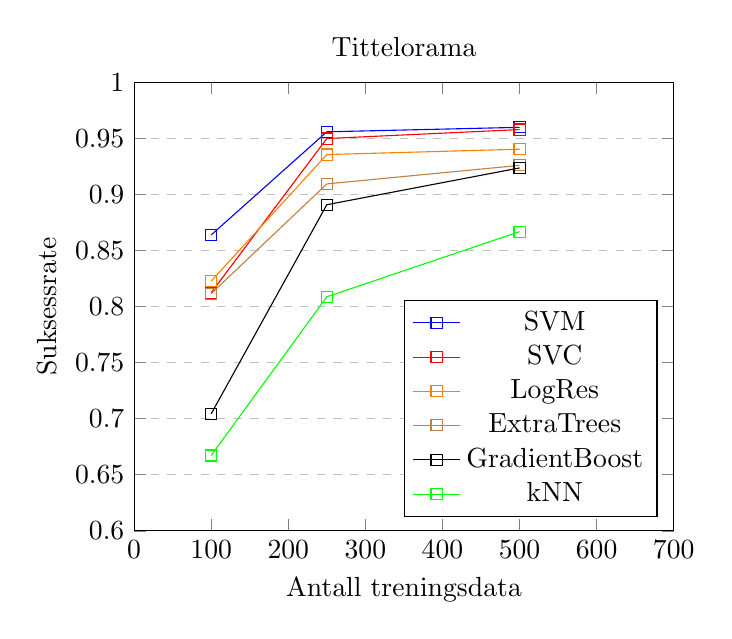
\begin{tikzpicture}
\begin{axis}[
    title={Tittelorama},
    xlabel={Antall treningsdata},
    ylabel={Suksessrate},
    xmin=0, xmax=700,
    ymin=0.6, ymax=1.0,
    xtick={0,100,200,300,400,500,600,700},
    ytick={0.6,0.65,0.7,0.75,0.8,0.85,0.9,0.95,1.0},
    legend pos=south east,
    ymajorgrids=true,
    grid style=dashed,
]
\addplot[
    color=blue,
    mark=square,
    ]
    coordinates {
    (100,0.864)(250,0.956)(500,0.96)
    };
\addplot[
    color=red,
    mark=square,
    ]
    coordinates {
    (100,0.8124)(250,0.95)(500,0.958)
    };
\addplot[
    color=orange,
    mark=square,
    ]
    coordinates {
    (100,0.8228)(250,0.9357)(500,0.94048)
    };
\addplot[
    color=brown,
    mark=square,
    ]
    coordinates {
    (100,0.8116)(250,0.9095)(500,0.92608)
    };
\addplot[
    color=black,
    mark=square,
    ]
    coordinates {
    (100,0.7044)(250,0.89095)(500,0.92376)
    };
\addplot[
    color=green,
    mark=square,
    ]
    coordinates {
    (100,0.6672)(250,0.8088)(500,0.86688)
    };
    
    \legend{SVM,SVC,LogRes,ExtraTrees,GradientBoost,kNN}
\end{axis}
\end{tikzpicture}
\label{figure:resultsgraf}
\caption{Resultatsutvikling for et utvalg algoritmer.}
\end{figure}

\subsection{Relatert arbeid}
{\color{red} 1-2 sider, utforskning av hva andre har gjort... Maskinlæring på sensordata fra gester (video)}

\subsection{Konklusjoner og videre arbeid}
Blablabla suksess!

I figur \ref{figure:resultsgraf} kan vi se at SVM'ene er i nærheten av 95\% allerede etter 250 treningseksempler og at de kun øker minimalt med 250 ekstra tilfeller. Dette tyder på at det trengs et svært antall ekstra treningseksempler for at algoritmene skal krype betydelig nærmere 100\%. De avanserte ExtraTrees og GradientBoost, benytter seg av kombinasjonsstrategier og flere teknikker. Det kan se ut som om spesielt GradientBoost kan fortsette å øke suksessraten betydelig med mer trening, men det er tvilsomt om den passerer SVM. Til sist nevnes k-næreste nabo, som begynner svakest av disse, men fremdeles har en sterk vekst mellom 250 og 500 tilfeller. Det hadde vært interessant å se utviklingen videre for denne enkle algoritmen.

Hva kan gjøres videre: online læring, flere gester (er det nyttig?), større egenskapvektor (enn 128) fordeler ulemper.




%%=========================================
\section{3 - asd}
%%=========================================
\subsection{asd}
asd
%%=========================================
\section{(< 2 (count sensors))}
%%=========================================
\subsection{Introduksjon (1 side)}

\subsection{Problemet (1 side)}

\subsection{Min idé (2 sider)}

\subsection{Detaljer (5 side)}

\subsection{Relatert arbeid (1-2 sider)}

\subsection{Konklusjoner og videre arbeid (0.5 side)}

\subsection{Kan vi forstå avanserte gester?}
asd
%%=========================================
\section{Et informasjonssystem drevet av kontekst}
%%=========================================
\subsection{Introduksjon / Problemet (1-2 sider)}

\subsection{Min idé (2 sider)}
{\color{red}PING: Et informasjonssystem for det smarte hjemmet bør være drevet av kontekst, ikke interaksjon.}

\subsection{Detaljer (5 sider)}

\subsection{Relatert arbeid (1-2 sider)}

\subsection{Konklusjoner og videre arbeid (0.5 side)}

%%=========================================
\section[Sammendrag]{Sammendrag og anbefalinger til fremtidig arbeid}
%%=========================================
\subsection{Sammendrag og konklusjoner}
asd
%%=========================================
\subsection{Anbefalinger til fremtidig arbeid}
asd

%%=========================================
%\appendix
%%This is Appendix A - Acronyms
%%=========================================

\chapter{Acronyms}
\begin{description}
\item[FTA] Fault tree analysis
\item[MTTF] Mean time to failure
\item[RAMS] Reliability, availability, maintainability, and safety
\end{description}
%%This is an Appendix
%%=========================================

\section{Additional Information}
This is an example of an Appendix. You can write an Appendix in the same way as a chapter, with sections, subsections, and so on.

%%=========================================
\subsection{Introduction}

%%=========================================
\subsubsection{More Details}
%%=========================================
\bibliographystyle{apa}
\addcontentsline{toc}{section}{\bibname}
\bibliography{refs}  
%%=========================================

\end{document}